\documentclass[12pt]{report}

\usepackage{fullpage,times}
\usepackage{graphicx}
\usepackage{enumitem}
\usepackage{amsmath}
\usepackage{authblk}
\usepackage{siunitx}
\usepackage{float}

\usepackage{algorithm}
\usepackage[noend]{algorithmic}
\setlength{\algorithmicindent}{2em}

\usepackage[nottoc]{tocbibind}
\renewcommand\bibname{References}

\usepackage[titletoc]{appendix}

\usepackage{setspace}

\graphicspath{{figures/}}

\setlist[enumerate]{
  labelindent=0pt,
  itemindent=0pt,
  leftmargin=*,
  noitemsep,
  topsep=0.25em
}
\setlist[itemize]{
  labelindent=0pt,
  itemindent=0pt,
  leftmargin=*,
  nosep
}

%%%%%%%%%%%%%%%%%%%%%%%%%%%%%%%%%%%%%%%%%%%%%%%%%%%%%%%%%%%%%%%%%%%%%%%%
%%%%%%%%%%%%%%%%%%%%%%%%%%%%%%%%%%%%%%%%%%%%%%%%%%%%%%%%%%%%%%%%%%%%%%%%
%%%%%%%%%%%%%%%%%%%%%%%%%%%%%%%%%%%%%%%%%%%%%%%%%%%%%%%%%%%%%%%%%%%%%%%%
\title{SMURF-seq: efficient short-read sequencing on long-read
  sequencers}
\author{Rishvanth K. Prabakar}
\affil{Quantitative and Computational Biology Section, \\
  Department of Biological Sciences, \\
  University of Southern California, \\
  1050 Childs Way, \\
  Los Angeles 90089, USA}

\date{April 21, 2020}

\begin{document}
%%%%%%%%%%%%%%%%%%%%%%%%%%%%%%%%%%%%%%%%%%%%%%%%%%%%%%%%%%%%%%%%%%%%%%%%
%%%%%%%%%%%%%%%%%%%%%%%%%%%%%%%%%%%%%%%%%%%%%%%%%%%%%%%%%%%%%%%%%%%%%%%%
%%%%%%%%%%%%%%%%%%%%%%%%%%%%%%%%%%%%%%%%%%%%%%%%%%%%%%%%%%%%%%%%%%%%%%%%
% \frontmatter
\maketitle
\doublespacing
\pagenumbering{roman}
\setcounter{page}{2}

%% Abstract
\addcontentsline{toc}{chapter}{Abstract}
%%%%%%%%%%%%%%%%%%%%%%%%%%%%%%%%%%%%%%%%%%%%%%%%%%%%%%%%%%%%%%%%%%%%%%%%
%%%%%                                                              %%%%%
%%%%% Abstract                                                     %%%%%
%%%%%                                                              %%%%%
%%%%%%%%%%%%%%%%%%%%%%%%%%%%%%%%%%%%%%%%%%%%%%%%%%%%%%%%%%%%%%%%%%%%%%%%
\chapter*{Abstract}
% SMURF-seq
We present SMURF-seq, a protocol to efficiently sequence short DNA
molecules on a long-read sequencer by randomly ligating them to form
long molecules.
%
Applying SMURF-seq using the highly portable and inexpensive Oxford
Nanopore MinION yields up to 30 fragments per read, providing an average
of 6.2 and up to 7.5 million mappable fragments per run, increasing
information throughput for read-counting applications.

% Copy number
Somatic copy number alterations play a significant role cancer, and can
be leveraged for diagnostic and personalized approaches to treatment.
% Drawbacks of high-throughput short-read
High-throughput short-read sequencing has been extremely efficient in
copy number profiling; however, its applicability depends on the
availability of instrument, and time to obtain profiles can vary from a
few days to weeks.
% Copy number profiling on MinION
We apply SMURF-seq on the MinION to generate copy number profiles and
demonstrate that multiple samples can be multiplexed in a single
sequencing run.  A comparison with profiles from Illumina sequencing
reveals that SMURF-seq attains similar accuracy.

% aligning SMURF-seq reads
A SMURF-seq read is aligned to the reference genome by splitting it into
its constituent fragments, each aligning to a distinct location in the
genome.
% Fragment identification
We define a score function for aligning a SMURF-seq read and describe an
approach to determine the optimal fragmentation of a read.

% big picture
More broadly, SMURF-seq expands the utility of long-read sequencers for
efficient short-read sequencing, enabling applications on long-read
sequencers that are currently only efficient on high-throughput
short-read sequencers.

%% Acknowledgements
\addcontentsline{toc}{chapter}{Acknowledgments}
%%%%%%%%%%%%%%%%%%%%%%%%%%%%%%%%%%%%%%%%%%%%%%%%%%%%%%%%%%%%%%%%%%%%%%%%
%%%%%                                                              %%%%%
%%%%% Acknowledgments                                             %%%%%
%%%%%                                                              %%%%%
%%%%%%%%%%%%%%%%%%%%%%%%%%%%%%%%%%%%%%%%%%%%%%%%%%%%%%%%%%%%%%%%%%%%%%%%
\chapter*{Acknowledgments}


\singlespacing

%% Table of contents and figures
\tableofcontents
\listoffigures

%%%%%%%%%%%%%%%%%%%%%%%%%%%%%%%%%%%%%%%%%%%%%%%%%%%%%%%%%%%%%%%%%%%%%%%%
%%%%%%%%%%%%%%%%%%%%%%%%%%%%%%%%%%%%%%%%%%%%%%%%%%%%%%%%%%%%%%%%%%%%%%%%
%%%%%%%%%%%%%%%%%%%%%%%%%%%%%%%%%%%%%%%%%%%%%%%%%%%%%%%%%%%%%%%%%%%%%%%%
% \mainmatter
\doublespacing

%% Introduction
%%%%%%%%%%%%%%%%%%%%%%%%%%%%%%%%%%%%%%%%%%%%%%%%%%%%%%%%%%%%%%%%%%%%%%%%
%%%%%                                                              %%%%%
%%%%% Chapter 1: Introduction                                      %%%%%
%%%%%                                                              %%%%%
%%%%%%%%%%%%%%%%%%%%%%%%%%%%%%%%%%%%%%%%%%%%%%%%%%%%%%%%%%%%%%%%%%%%%%%%
\chapter{Introduction}
\label{ch1}

In the last decade, massively parallel high-throughput short-read
sequencing has revolutionized the efficiency and breadth of applications
for DNA sequencing \citep{kircher2010high}.  These high-throughput
sequencing methods produce millions to billions of short reads in a
single run, and have led to the development of many applications that
depend on ``read-counting'' to measure the abundance of specific
sequences in a sample. Examples include RNA-seq, ChIP-seq, and
whole-genome copy number profiling.

Recently, long-read technologies have been developed that are filling
the gap left by short-read sequencers in applications such as genome
assembly \citep{jain2018nanopore,loman2015complete}, which benefit from
connecting more distant sequences within a contiguous molecule. Among
these, the MinION instrument, from Oxford Nanopore Technologies, is
highly portable and inexpensive and has shown its unique value for
analysis outside of central sequencing facilities \citep{quick2016real}.
Long-read sequencers such as the MinION typically produce vastly fewer
reads from a sequencing run, and are therefore less efficient in
applications that use sequenced reads purely as a means to count
molecules. However, these technologies have the enormous advantage of
operating in near real-time, with a turnaround time that can be measured
in hours for some applications, rather than days or weeks.

Copy number alteration (CNA) has been used successfully to understand a
variety of diseases \citep{fanciulli2010gene} -- notably cancers, which
exhibit both extreme variation and recurrent trends that can be used for
diagnostics and personalized approaches to treatment. For example, the
amplification and loss of certain genes, such as \textit{RB1} deletion
and \textit{MYCN} amplification in retinoblastoma, can be prognostic or
even predictive for treatment \citep{berry2017potential}.
High-throughput short-read sequencing has been extremely effective in
copy number profiling of cancers \citep{chiang2009high}, including
profiling single tumor cells \citep{navin2011tumour}. However, for many
potential users, the efficiency of high-throughput short-read sequencing
in CNA analysis is determined by the availability of instruments and the
need for heavy multiplexing to hit a reasonable cost per profile. A
sequencing core is typically involved and an individual profile must
wait for a ``full'' run before it can be processed. The MinION sequencer
has an accessible buy-in and is easy to use. Unfortunately, the MinION
has optimal nucleotide throughput when producing reads that are orders
of magnitude longer than needed for CNA profiling.

To make full use of the advantages offered by the MinION sequencer, we
introduce sampling molecules using re-ligated fragments (SMURF)-seq, a
protocol to efficiently sequence short DNA molecules on a long-read
sequencer \citep{prabakar2019smurf}. The strategy of SMURF-seq is to
concatenate short fragments into very long molecules ($\sim$8 kb) prior
to sequencing. After (or possibly concurrent with) sequencing, the
SMURF-seq reads are mapped to the reference genome by splitting them
into their constituent fragments, each aligning to a distinct location
in the genome.
%
We demonstrate the utility of SMURF-seq with the low-cost MinION
sequencer to obtain data similar to that expected from typical
short-read sequencing, and generated high-quality copy number profiles
from this output.

More broadly, SMURF-seq is an approach for efficient short-read
sequencing, as required for read-counting, on long-read sequencing
machines. Here, we describe the details of the SMURF-seq approach; both
the SMURF-seq protocol prior to sequencing and mapping the sequenced
SMURF-seq reads. This study is organized as follows:

%%% Summary of chapters
% Chapter 2: Background
In the second chapter, we review the relevant background.  First, we
discuss the concept of nanopore sequencing and summarize its history,
the MinION sequencing instrument and its utility, library construction
methods, and sequencing on these machines.
%
Then, we discuss the copy number profiling and its implications in
diversity and disease; especially its involvement in cancer, and the
utility of copy number analysis in understanding the biology of cancer
and diagnostic evaluation of tumors. We summarize methods and
computational approaches for generating copy number profiles.
%
Finally, we discuss prior protocols that are similar in spirit to
SMURF-seq, including SAGE and its variants, SMASH, and Concat-seq.

% Chapter 3: SMURF-seq
In the third chapter, we describe the details of the SMURF-seq approach
and demonstrate the accuracy of this approach for CNA profiling.  We
start with a discussion of sequencing long-reads or short-reads directly
for read-counting on nanopore machines, and the merits and limitations
of these methods.
%
Then, we introduce the SMURF-seq protocol for efficient short-read
sequencing on long-read machines; SMURF-seq combines the merits of
sequencing long or short reads directly while alleviating the
limitations.
%
We demonstrate that SMURF-seq generates higher read-counts from a
sequencing run in comparison to these other methods, the copy number
profiles generated with SMURF-seq are as accurate as profiles generated
using an Illumina platform, multiple samples can be multiplexed and
sequencing in the same sequencing run, and the reads generated in the
first few minutes of sequencing are sufficient to generate accurate
profiles.
%
Finally, we provide future directions for further improving the
efficiency and expanding the utility of SMURF-seq.

% Chapter 4: Mapping SMURF-seq reads
The fourth chapter is dedicated to algorithmic and statistical aspects
of mapping SMURF-seq reads. We discuss the challenges associated with
mapping SMURF-seq reads as the fragments get shorter.
%
We introduce the fragment identification problem as a way of identifying
fragment boundaries and estimating the optimal number of fragments on a
SMURF-seq read.
%
Next, we define a score function for aligning SMURF-seq reads and
describe algorithms to find fragment boundaries on a read such that the
score is maximized.
%
Then, we determine the null distribution of aligning a SMURF-seq read
generated at random to calculate a p-value for a particular
fragmentation of a read. We use these p-values to determine the optimal
number of fragments on a read.
%
Finally, we suggest future directions of aligning SMURF-seq reads with
short fragments to large reference genomes.

% Chapter 5: Conclusion
We conclude this study by highlighting our vision of using the SMURF-seq
approach for short-read sequencing on long-read sequencers; we envision
that with further optimizations to SMURF-seq, to both the protocol and
mapping algorithms, would drive down the cost of sequencing and broaden
the applications of long-read sequencers.

%% Background
%%%%%%%%%%%%%%%%%%%%%%%%%%%%%%%%%%%%%%%%%%%%%%%%%%%%%%%%%%%%%%%%%%%%%%%%
%%%%%                                                              %%%%%
%%%%% Chapter 2: Background                                        %%%%%
%%%%%                                                              %%%%%
%%%%%%%%%%%%%%%%%%%%%%%%%%%%%%%%%%%%%%%%%%%%%%%%%%%%%%%%%%%%%%%%%%%%%%%%

\chapter{Background}
\label{ch2}

%%%%%%%%%%%%%%%%%%%%%%%%%%%%%%%%%%%%%%%%%%%%%%%%%%%%%%%%%%%%%%%%%%%%%%%%
%%%%%%%%%%%%%%%%%%%%%%%%%%%%%%%%%%%%%%%%%%%%%%%%%%%%%%%%%%%%%%%%%%%%%%%%
%%%%%%%%%%%%%%%%%%%%%%%%%%%%%%%%%%%%%%%%%%%%%%%%%%%%%%%%%%%%%%%%%%%%%%%%
\section{Nanopore sequencing}


%%%%%%%%%%%%%%%%%%%%%%%%%%%%%%%%%%%%%%%%%%%%%%%%%%%%%%%%%%%%%%%%%%%%%%%%
%%%%%%%%%%%%%%%%%%%%%%%%%%%%%%%%%%%%%%%%%%%%%%%%%%%%%%%%%%%%%%%%%%%%%%%%
%%%%%%%%%%%%%%%%%%%%%%%%%%%%%%%%%%%%%%%%%%%%%%%%%%%%%%%%%%%%%%%%%%%%%%%%
\section{Copy number variation and profiling}


%%%%%%%%%%%%%%%%%%%%%%%%%%%%%%%%%%%%%%%%%%%%%%%%%%%%%%%%%%%%%%%%%%%%%%%%
%%%%%%%%%%%%%%%%%%%%%%%%%%%%%%%%%%%%%%%%%%%%%%%%%%%%%%%%%%%%%%%%%%%%%%%%
%%%%%%%%%%%%%%%%%%%%%%%%%%%%%%%%%%%%%%%%%%%%%%%%%%%%%%%%%%%%%%%%%%%%%%%%
\section{Prior protocols based on concatenating DNA molecuels}
% SAGE and its variants

% SMASH

% concat-seq

%% SMURF-seq
%%%%%%%%%%%%%%%%%%%%%%%%%%%%%%%%%%%%%%%%%%%%%%%%%%%%%%%%%%%%%%%%%%%%%%%%
%%%%%                                                              %%%%%
%%%%% Chapter 3: SMURF-seq                                         %%%%%
%%%%%                                                              %%%%%
%%%%%%%%%%%%%%%%%%%%%%%%%%%%%%%%%%%%%%%%%%%%%%%%%%%%%%%%%%%%%%%%%%%%%%%%
\chapter{Sampling molecules using re-ligated fragments (SMURF)-seq}
\label{ch3}


%%%%%%%%%%%%%%%%%%%%%%%%%%%%%%%%%%%%%%%%%%%%%%%%%%%%%%%%%%%%%%%%%%%%%%%%
%%%%%%%%%%%%%%%%%%%%%%%%%%%%%%%%%%%%%%%%%%%%%%%%%%%%%%%%%%%%%%%%%%%%%%%%
%%%%%%%%%%%%%%%%%%%%%%%%%%%%%%%%%%%%%%%%%%%%%%%%%%%%%%%%%%%%%%%%%%%%%%%%
\section{Naive approaches to read-counting on nanopore machines}
%% Long read approach
Copy number profiling, and read-counting in general, can be done on
nanopore sequencers with long reads ($\sim$8kb) following the standard
sequencing procedure.
% Advantages of long read sequencing
Since nanopore machines are optimized for long read sequencing, this
method has the advantage of using any standard library preparation
protocol that are commercially available. Further, technical
nucleotides, such as sequencing adapters and barcodes, are sequenced one
(or twice) every $\sim$8k bases, thus the fraction of time a nanopore
spends sequencing technical nucleotides is low.
% Disadvantages of long read sequencing
However, read-counting applications do not benefit from longer reads
beyond what is necessary for unique mapping to the reference genome. In
these applications, for any fixed number of nucleotides sequenced, more
information would be obtained if those nucleotides are organized as more
DNA molecules, rather than longer contiguous fragments.

%% Short read sequencing
An alternate approach to read-counting is to sequence short reads
($\sim$150 bp) directly on a nanopore sequencer.
%% Advantages of short read sequencing
In general, for a given sample of DNA, a nanopore instrument will
generate more reads if the corresponding molecules are shorter.  Once a
molecule is loaded into a pore, the time spent sequencing is less for
shorter reads. In addition, for a fixed amount of DNA, shorter molecules
result in higher molar concentration when loaded onto the machine,
increasing the rate at which each pore captures molecules
\citep{muthukumar2010theory,wanunu2008dna}. Therefore, sequencing short
reads on a nanopore machine would generate more reads from a sequencing
run than sequencing long reads.
%% Disadvantages of short read sequencing
However, sequencing short reads requires ad-hoc modifications to the
library preparation protocol as these are optimized for longer
molecules.  Moreover, technical nucleotides are sequenced every
$\sim$150bp, increasing the fraction of time a nanopore sequences the
technical bases.

%% SMURF-seq approach
SMURF-seq approach combines the advantages of both of these methods
while alleviating the drawbacks by using a nanopore instrument as
intended for long-read sequencing, while generating the desired short
fragments. Using the SMURF-seq approach we generate higher read counts
per run than sequencing long or short molecules directly.


%%%%%%%%%%%%%%%%%%%%%%%%%%%%%%%%%%%%%%%%%%%%%%%%%%%%%%%%%%%%%%%%%%%%%%%%
%%%%%%%%%%%%%%%%%%%%%%%%%%%%%%%%%%%%%%%%%%%%%%%%%%%%%%%%%%%%%%%%%%%%%%%%
%%%%%%%%%%%%%%%%%%%%%%%%%%%%%%%%%%%%%%%%%%%%%%%%%%%%%%%%%%%%%%%%%%%%%%%%
\section{SMURF-seq approach to read counting}
%% SMURF-seq concept
The SMURF-seq protocol involves cleaving genomic DNA into short
fragments, with length just sufficient for an acceptable rate of
uniquely mapping fragments in the reference genome.  These fragmented
molecules are then randomly ligated back together to form artificial
long DNA molecules, as required for long-read sequencing. The long
re-ligated molecules are sequenced following the standard MinION library
preparation protocol. After (or possibly concurrent with) sequencing,
the SMURF-seq reads are mapped to the reference genome in a way that
simultaneously splits them into their constituent fragments, each
aligning to a distinct location in the genome (Fig.~\ref{smurf}).

\begin{figure}[b!]
\centering
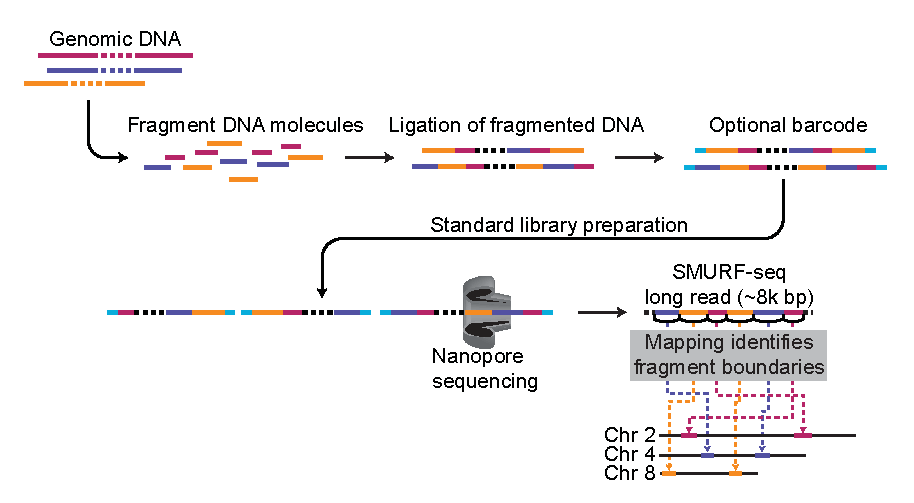
\includegraphics{smurf.pdf}
\caption{
  SMURF-seq efficiently sequences short fragments of DNA for
  read-counting applications with a reference genome on long-read
  sequencers, and yields up to 30 countable fragments per sequenced read.
  SMURF-seq sequences short DNA molecules by generating long concatenated
  molecules from these.  SMURF-seq reads are aligned by splitting them
  into multiple fragments, each aligning to a distinct region in the
  genome.}
\label{smurf}
\end{figure}


\begin{figure}[t!]
\centering
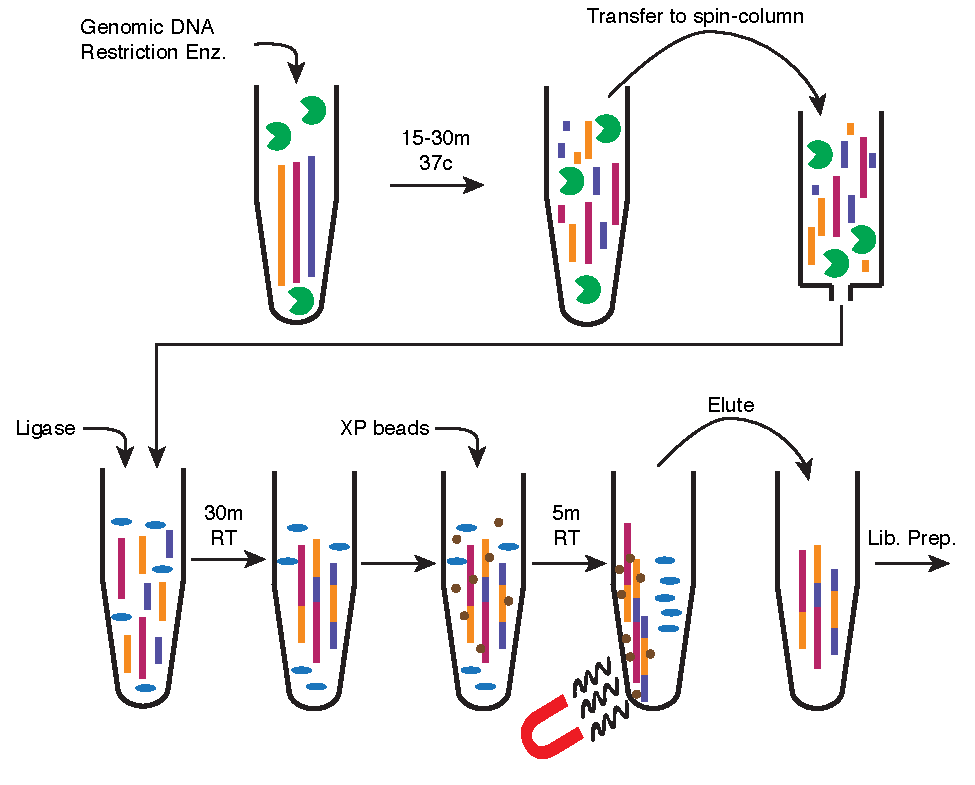
\includegraphics{ch3_fig2.pdf}
\caption{Schematic of SMURF-seq protocol. SMURF-seq consists of four
  steps: restriction enzyme digestion, spin-column clean-up, re-ligation
  of fragmented DNA, and Ampure XP beads clean-up.}
\label{protocol}
\end{figure}

%% Description of SMURF-seq protocol
More specifically, genomic DNA was fragmented using restriction enzymes
and ligated with T4 DNA ligase, with clean-up steps in between.
SMURF-seq protocol is completely enzymatic and takes less than 90
minutes to complete (Fig.~\ref{protocol}).  The details of these steps
are given below:
%%
\begin{enumerate}
\item Restriction enzyme digestion: restriction enzymes recognize
  and cleave specific DNA sequences, typically producing sticky-ended DNA
  molecules.
  %% choice of re used
  The choice of restriction enzyme used is primarily dependent on the
  size of the fragmented molecules produced. Based on the downstream
  application, they could also be influenced by other factors such as any
  bias they could introduce.
  %% advantages
  An advantage of using restriction enzymes to fragment DNA molecules,
  over other fragmentation techniques, is that the fragmented molecules
  have a uniform ends (either overhangs with the same sequence or
  blunt-ends) and are thus compatible for ligation without an end-repair
  step in between.

\item Clean-up: the reaction containing the restriction
  enzymes and the fragmented DNA molecules is cleaned to wash out the
  enzymes and retain the DNA molecules. The choice of clean-up kit used, also
  determines the length of the DNA molecules that are retained. We used a
  spin-column based clean-up that typically retains molecules that are over
  $\sim$70 bp. However, other clean-up kits, such as bead-based kits,
  could also be used at this step.

\item Re-ligation: fragmented DNA molecules with uniform ends are
  ligated at random with T4 DNA ligase enzymes.
  %% influence of time
  The most important factor in a ligation reaction is the
  concentration of compatible DNA ends \citep{dugaiczyk1975ligation}. At
  high concentrations, the chances are higher for ligation between two
  molecules than a molecule self-ligating. At low concentrations, the
  chances are higher for self-ligation.
  %%
  Thus, the main consideration during the ligation step is the
  duration of the ligation reaction, as the molar concentration of DNA
  molecules decrease with time. Too little time would lead to insufficient
  ligation, resulting in molecules of length that do not achieve optimal
  SMURF-seq efficiency. On the other extreme, too much time would result
  in circular molecules that are incompatible with the most downstream
  library preparation process. A typical ligation reaction would contain
  both short and circularized molecules, and achieving a balance between
  these determines the efficiency of SMURF-seq.
  %%
  Other factors such as the temperature and buffer contents also affect
  the ligation process.
  %% our experiments
  In our experiments, the ligation reaction was performed at a DNA
  concentration of \SI{25}{\nano\gram}$/$\SI{}{\micro\litre}
  (\SI{500}{\nano\gram} of DNA in \SI{10}{\micro\litre} nuclease free
  water and \SI{10}{\micro\litre} DNA ligase) for \SI{30}{\minute}.

\item Bead-based clean-up: the reaction containing the ligase enzymes and
  ligated DNA molecules is cleaned to retain only the ligated molecules. We
  used a bead-based clean-up at this step to avoid damage to long DNA
  molecules that are typical of spin-column based methods.
\end{enumerate}

%% Library construnction using standard protocols
DNA molecules that are resultant of the SMURF-seq protocol are long DNA
molecules that are several kilo-bases long, and therefore, any standard
library preparation kits that are available for nanopore machines can be
used with SMURF-seq molecules. These molecules can also be barcoded
with one (or two) barcode sequences per molecule. Thus, the SMURF-seq
approach overcomes the disadvantages of sequencing long or short DNA
molecules directly on a nanopore machine for read-counting applications,
and improves its efficiency for read-counting applications.

We also tested dsDNA Fragmentase enzymes (New England Biolabs) and
acoustic shearing (Covaris) to fragment DNA. However, these methods
require an additional end-repair step after fragmentation and the
ligated molecules failed to reach the lengths we obtained by using
restriction fragmentation.

\begin{figure}[t!]
\centering
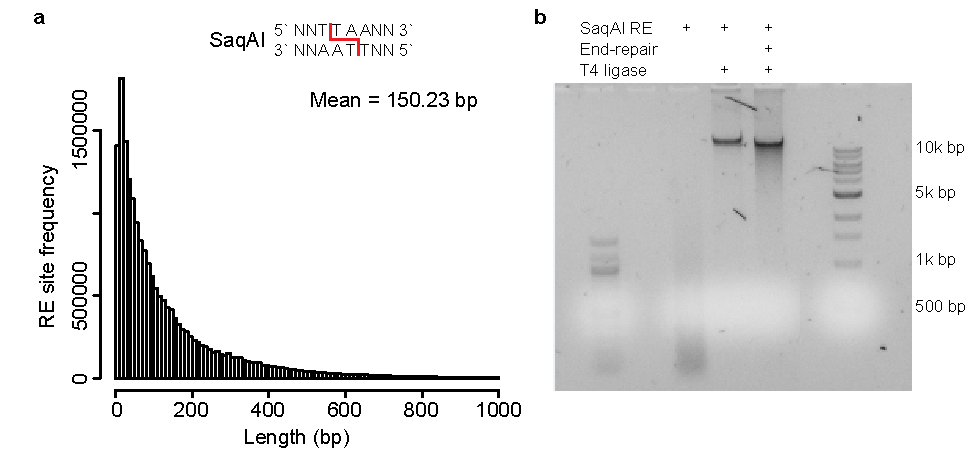
\includegraphics{ch3_fig3.pdf}
\caption{Restriction digestion and ligation of DNA molecules.
  (a) Distribution of length between restriction sites computed
  by measuring the distance between the recognition sites on the human
  reference genome. SaqAI recognizes the sequence TTAA and leaves a 2 bp
  overhang.
  (b) Negative gel image of fragmented and ligated normal diploid DNA
  using SaqAI restriction enzyme and T4 DNA ligase.  Sticky-end and
  blunt-end ligation (by end-repair) of fragmented DNA are shown, and
  both yield ligated molecules of approximately the same length.}
\label{re_frag}
\end{figure}

%% The sepecifics of our experiment
%% restriction digestion
In our applications, we used SaqAI restriction enzyme, which recognizes
the sequence TTAA and produces molecules with mean lengths of 150.2 bp
(Fig.~\ref{re_frag}a).
%% re-ligation
The fragmented DNA molecules are then ligated randomly to form longer
molecules using T4 DNA ligase enzyme (Fig.~\ref{re_frag}b).
%
In our experiments, the resulting long DNA molecules were sequenced
using the Oxford Nanopore Technologies 1D DNA by ligation kit
(SQK-LSK108) or the rapid sequencing kit (SQK-RAD003) following the
standard manufacturers protocol. We also multiplexed samples using the
1D native barcoding genomic DNA kit (EXP-NBD103) followed by library
preparation using the 1D DNA by ligation kit.
%
The detailed SMURF-seq protocol is given in Appendix~\ref{appendA}.


%%%%%%%%%%%%%%%%%%%%%%%%%%%%%%%%%%%%%%%%%%%%%%%%%%%%%%%%%%%%%%%%%%%%%%%%
%%%%%%%%%%%%%%%%%%%%%%%%%%%%%%%%%%%%%%%%%%%%%%%%%%%%%%%%%%%%%%%%%%%%%%%%
%%%%%%%%%%%%%%%%%%%%%%%%%%%%%%%%%%%%%%%%%%%%%%%%%%%%%%%%%%%%%%%%%%%%%%%%
\section{Mapping SMURF-seq reads}
The reads sequenced using SMURF-seq can be mapped to a reference genome
by first identifying short matches within the reads, corresponding to
parts of the individual fragments, and then extending those to locate
fragment boundaries.
%
As currently implemented, SMURF-seq fragments are longer than
$\sim$150bp, and mapping these reads is is handled nicely using the
seed-and-extend paradigm implemented in many existing long-read mapping
tools. Although none of these tools were designed to align SMURF-seq
reads, several long read aligners include steps designed for split-read
alignment, which can be leveraged from aligning SMURF-seq reads.

%% TODO: Need to expand on the four steps below
Aligning SMURF-seq reads with long-read mapping tools involve variations
of the following steps:
%% Steps involved in mapping SMURF-seq reads
\begin{itemize}
\item Identifying seeds: Mapping tools have a step of identifying seeds,
  which are short exactly matching parts of the read with parts of the
  reference genome. Choices in how seeds are defined and used are often
  made for mapping speed. The total size of SMURF-seq data sets is
  currently (relatively) small, so speed is not our primary concern. We
  favor the most sensitive seed strategy, but depending on implementation
  too many seed hits could lead to ambiguity later in the mapping process.
\item Chaining seeds: The identified seeds are further extended into
  proto alignments, and filtered to avoid aligning potentially false
  positive seed hits.
\item Aligning within the chains: In this stage a Smith-Waterman
  alignment is performed, typically allowing users to specify a mismatch
  penalty along with penalties for both gap-open and gap-extend.
\item Selecting best alignments: When high-scoring alignments overlap
  within a read, one of them (or both) could be trimmed or one is selected
  and the other discarded. The choices made here could lead to discarding
  entire fragments.
\end{itemize}

%% parameter options
Mapping tools have several parameter options, in general, these are
related to: (1) the seeding and chaining algorithm used by the
individual tool.  (2) The Smith-Waterman alignment scores, i.e. the
match score, and the mismatch and indel penalty. The seeding and
chaining parameters control the number of proto alignments that are
further refined by aligning parts of the read to the reference genome
using the specified alignment scores.

%% Importance of picking the optimal SW score
The Smith-Waterman alignment score used to align fragments to the
reference genome is crucial for determining the optimal fragment length.
On one extreme, a match score of 1 with a mismatch and indel penalty of
0 will result in one identified fragment covering the entire read and
mapping perfectly, but will always map ambiguously. On the other
extreme, a match score of 1 with a mismatch and indel penalty of
$-\infty$ will result in any mismatch or indel on the read to be
considered as a fragment boundary. Therefore to align SMURF-seq reads,
we need to determine optimal alignment scores to use.

We evaluated mapping tools on simulated SMURF-seq data generated by
concatenating random fragments from real Oxford Nanopore reads. This
emulates idealized SMURF-seq reads. Within the simulated reads, the
boundaries of each fragment are known \textit{a priori}, as are their
mapping locations when in the context of their original long reads. We
used this information to evaluate mapping tools in terms of (1) how well
they identify fragments purely for the purpose of counting molecules,
which is the primary information used in CNV analysis, and (2) how well
they identify individual mapping bases within reads. After mapping these
reads, we calculated precision and recall for identifying both the
correct fragment locations, and the individual mapping bases within the
fragments (i.e. the correct fragment boundaries). Using this simulation
setup, we determined the optimal Smith-Waterman alignment score for use
with SMURF-seq reads.

\subsection{Simulating SMURF-seq reads to evaluate mapping programs}
To test these mapping tools, we chose to create simulated reads with the
technical characteristics we expect in idealized SMURF-seq data. We
first selected a fragment length $\ell$ and a number $k$ of fragments
per read. Then, for a given WGS nanopore data set, we took the set of
mapped long reads as determined by BWA-MEM (with \texttt{-x ont2d}
option).
Each of the mapped reads was split into fragments of length $\ell$ (with
a random offset of $0$ to $\ell-1$ at the start of the long read). Each
fragment was validated by requiring that it did not overlap a deadzone
in the genome (as determined by the deadzone program available from
https://github.com/smithlabcode/utils for 40 bp). The reason for
excluding deadzones is that even when a short fragment has a ``known''
mapping location when it is part of a longer read, we cannot compare its
reported mapping location as a short fragment with that known location,
since we expect any good mapping algorithm to identify that the fragment
maps ambiguously. Among these validated fragments, subsets of $k$ were
sampled uniformly at random and concatenated (in random order and
orientation) to form simulated SMURF-seq reads.

The first and last fragments in a read should be slightly easier to
identify and map than the rest, since one of their boundaries is
known. Using the above procedure, we select $k=20$ so that the
simulated reads have a sufficient number of fragments to eliminate the
influence of the first and last fragments in each read on the
results. There is no need to have large $k$ otherwise.

By lowering $\ell$ and making the fragments shorter, the task of
mapping the fragments becomes more challenging. Real SMURF-seq reads
have fragment lengths determined by restriction site density, size
selection and other aspects of the experiments. But in testing mapping
algorithms and optimizing parameters, there is no disadvantage to
making the task more challenging. We only need to be able to
distinguish the relative performance of different mapping tools and
parameter combinations. Real SMURF-seq reads have varying fragment
lengths, but in evaluating mapping tools, there is no need to
randomize fragment lengths. None of the algorithms we evaluated are
capable of either deducing or leveraging the fact that all simulated
fragments have the same length. We selected $\ell = 100$, which
begins to challenge the various mapping strategies. These values of
$\ell$ are slightly lower than the average in real SMURF-seq data.


\subsection{Evaluating performance using simulated SMURF-seq reads}
Within the simulated reads, the boundaries of each fragment are known
\textit{a priori}, as are their mapping locations. We used this
information to evaluate mapping tools in terms of (1) how well they
identify fragments purely for the purpose of counting molecules, which
is the primary information used in CNV analysis, and (2) how well they
identify individual mapping bases within reads. The latter criteria
becomes important in challenging cases and will be increasingly
important as fragment sizes are reduced.

Performance on identifying fragments: After mapping these simulated
reads, each mapping result is called a predicted fragment. Each
predicted fragment is considered a positive prediction, and we assume
an arbitrary order over positive predictions. A positive prediction is
a true positive if:
\begin{itemize}
\item The predicted fragment maps uniquely.
\item The mapping locations of at least half the bases in the
  predicted fragment are equal to the original mapping locations for
  those bases, and those bases are all part of the same original
  fragment (we assume that it is unlikely for two fragments on a simulated
  read to have the same mapping location but opposite orientation, and thus
  do not check for the orientation of a fragment). In this case, we say the
  predicted fragment is associated with that original fragment.
\item The predicted fragment is the first among predicted fragments
  associated the same original fragment.
\end{itemize}
False positives are predicted fragments that are not true positives. Any
original fragment with no associated predicted fragment is a false
negative. These criteria penalize splitting one original fragment or
merging two original fragments. By defining true positives, false
positives and false negatives we are able to calculate precision,
recall, and F-score for a particular mapping strategy.
%%%

Performance on identifying individual mapping bases: After mapping
simulated reads, each mapping result is decomposed into individual
nucleotides and associated with a location in the genome. Those
locations are retained. We keep multiplicities, so when two mapped
fragments overlap in the genome we count certain nucleotides twice.
These are the predicted positive bases in the reference.  The condition
positive bases are those known \textit{a priori} from the simulation.
The original fragment mapping locations may overlap in the reference
genome, leading to multiplicities in the condition positive bases, but
with low probability. The true positives are the intersection of the
condition positive and the predicted positive bases. When there are
multiplicities of mapped fragments and simulated fragments overlapping
the same bases in the reference genome, this is determined by taking the
smaller of the two values. After removing the true positives bases, the
remaining predicted positive bases are false positives, and the
remaining condition positive bases are false negatives. These criteria
penalize mapping approaches that do not cover the entire simulated
SMURF-seq reads, and also penalize approaches that predict fragments
that overlap within the read. The true positives, false positives, and
false negatives here allow us to assign precision and recall in terms of
individual bases and corresponding F-scores. Although the reference
bases for both predicted positive and condition positive could involve
multisets, since our simulations used relatively low coverage this
almost never happened.

To generate simulated reads we used the standard long reads from four
sequencing runs (Flowcell ID: FAB42704, FAB42810, FAB49914, and
FAF01253) in the public dataset available at \\
https://github.com/nanopore-wgs-consortium/NA12878/blob/master/Genome.md
\citep{jain2018nanopore,jain2018nanopore_git}. We downloaded the raw data
from EBI (Run accession: ERR2184696, ERR2184704, ERR2184712, and
ERR2184722) and base-called these with Guppy (version: 2.3.5).


\subsection{Initial selection of mapping tools}
We tested the following mapping tools: BWA-MEM\citep{li2013aligning},
Minimap2\citep{li2018minimap2}, LAST\citep{kielbasa2011adaptive},
GraphMap\citep{sovic2016fast}, BLASR\citep{chaisson2012mapping},
rHAT\citep{liu2015rhat}, and LAMSA\citep{liu2017lamsa}. These were
selected either because they are known to perform well on certain
mapping tasks or have unique properties that plausibly could help in
mapping SMURF-seq reads. We tested each of these using default
parameters on simulated reads and downsampled real SMURF-seq
reads (data not shown). Among these BWA-MEM, Minimap2, and LAST had
higher accuracy on simulated data, and the other tools identified at
most 15 fragments per read on real data. Thus, we explored performance
of BWA-MEM (0.7.17), LAST (963), and Minimap2 (2.15) in more detail,
varying parameters to improve performance.

We remark that none of these tools were designed to map SMURF-seq reads;
results we report here do not reflect the overall performance of the
various mapping tools, only that the three aforementioned tools happened
to perform relatively well on a task for which they were not directly
designed for.


\subsection{Determining the optimal Smith-Waterman score for
  SMURF-seq reads}
%% alignment score grid
In order to determine the optimal alignment score, we kept the seeding
related parameters constant, and varied the alignment score combinations
to perform a grid search. We varied the mismatch penalty from 1 to 6,
gap open penalty from 0 to 4, and gap extend penalty form 1 to 4.  The
match score was fixed at 1. Thus for each tool we tested 120 ($6 \times
5 \times 4$) combinations of alignment scores.

%% seeding parameter for each tool
The seeding and chaining related parameters for each tool was set at
follows (along with the four alignment scores):
\begin{itemize}
\item BWA-MEM: \texttt{-x ont2d -k 12 -W 12 -T 30}
\item Minimap2: \texttt{-w 1 -m 10 -s 30}
\item LAST (NEAR): \texttt{lastal -Q0 -e 20} and \texttt{last-split -m 1 -s 30}
\end{itemize}
We set the seeding and chaining parameters in a liberal manner to allow
for higher sensitivity than the default parameter of each tool, and
the minimum alignment score to output was set at 30.

%% selecting the best alignment parameter
After aligning the simulated reads, we calculated the average precision
and recall, each for the mapped fragment locations and nucleotides, for
the four datasets. The F-score was computed for each, and the mean of
the F-scores was used to determine the optimal alignment parameter for
each tool. Based on these results BWA-MEM outperformed other tools for
aligning SMURF-seq reads. BWA-MEM performed best with a mismatch, open,
and extension penalty of 2, 1, 1 respectively.

%% Zooming in on the grid for BWA
To further refine the optimal alignment parameter for BWA-MEM, we
aligned the simulated reads with parameter values around the value
described above with a higher resolution. We varied the mismatch penalty
from 1.5 to 2.5, and open and extend penalties from 0.5 to 1.5 in
increments of 0.25.
%
However, BWA-MEM does not accept floating point values for alignment
score parameters. To overcome this, we scaled the alignment score
proportionately to have integer values, i.e we varied the mismatch
penalty from 6 to 10, open and extend penalties from 2 to 6, and fixed
the match score at 4 (125 combinations).
%
Based on these results, the highest accuracy was obtained with the
mismatch, open, and extension penalty of 2.5, 1.5, 0.75 respectively
(corresponding scaled values are 10, 6 and 3). We used these optimal
alignment scores for mapping real SMURF-seq read, and all the CNV
profiles presented are based on these.


%%%%%%%%%%%%%%%%%%%%%%%%%%%%%%%%%%%%%%%%%%%%%%%%%%%%%%%%%%%%%%%%%%%%%%%%
%%%%%%%%%%%%%%%%%%%%%%%%%%%%%%%%%%%%%%%%%%%%%%%%%%%%%%%%%%%%%%%%%%%%%%%%
%%%%%%%%%%%%%%%%%%%%%%%%%%%%%%%%%%%%%%%%%%%%%%%%%%%%%%%%%%%%%%%%%%%%%%%%
\section{Generating higher fragment counts with SMURF-seq}
%% Long read sequencing
A typical Oxford MinION sequencing run generates approximately 500k
reads (length $\sim$8 kb) \citep{jain2018nanopore,tyson2018minion} using
the standard library preparation and sequencing protocols. Several
studies have used these long reads for copy number profiling
\citep{euskirchen2017same,magi2019nano}.
%% Short read sequencing
We tested the ability of the Oxford MinION instrument to sequence short
DNA molecules by sequencing restriction enzyme (SaqAI) digested normal
diploid genome.  The sequencing run produced 2.58 million reads with a
mean read length of 630.93 bp.
%% SMURF-seq
Using the same instrument, with SMURF-seq, we report here an average of
6.2 million mapped fragments per run, which is substantially more
fragments than directly sequencing long or short reads directly.
Further, the SMURF-seq approach generated fragments at a substantially
faster rate than sequencing short molecules directly
(Fig.~\ref{frag_time}).

\begin{figure}[t!]
\centering
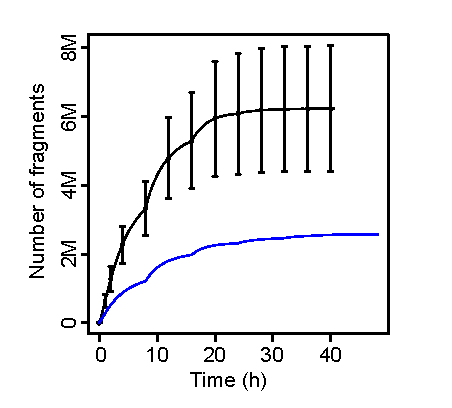
\includegraphics{frag_time.pdf}
\caption{SMURF-seq generates fragments at a faster rate than sequencing
short molecules directly. Number of fragments obtained from reads
plotted as a function of  sequencing time. For SMURF-seq, the average
number of fragments from runs using the 1D sequencing by ligation kits
are plotted (Error bars indicate one standard deviation). For short-read
sequencing run, each read is considered as one fragment.}
\label{frag_time}
\end{figure}

%% Why does SMURF-seq perform better?
% pore reload time
The most important factor in the performance of SMURF-seq over
sequencing short molecules directly is that sequencing concatenated
fragments effectively eliminates the pore reload time for all but the
first fragment in each read. However, there are a variety of additional
factors that favor further optimization of the approach employed by
SMURF-seq.
% sequences fewer technical bases
First, reduction of resources spent on technical nucleotides: SMURF-seq
uses a single barcode and sequencing adapter per read consisting of
multiple fragments; sequencing short reads uses one barcode and adapter
per fragment, adding approximately 50 bases to each fragment. This
increases the time to sequence each short read. In sequencing short
reads, as the reads get shorter the time consumed by these technical
bases increases. In SMURF-seq, sequencing either shorter fragments in
fixed length reads, or longer reads containing fragments of fixed
average length, both reduce the time consumed sequencing these technical
bases.
%
In the limit, assuming 100bp DNA fragments, sequencing those fragments
as short-reads corresponds to 33\% technical nucleotides; for SMURF-seq,
the portion of technical nucleotides remains low.
% Nanopores sequence at full speed
Second, more nucleotides sequenced at full speed: We observed that the
speed of sequencing was lower when sequencing short molecules. For
example, the average sequencing speed was 315.54 bases per second for
sequencing the diploid genome without SMURF-seq, and 400.29 bases per
second when sequencing using SMURF-seq on the MinION sequencer.
% Compatible with all library prep kits
Third, leveraging optimizations to long-read protocols: The rapidly
evolving nanopore library construction kits are continually optimized
for long-read sequencing, and would likely require significant ad-hoc
modifications to optimize sequencing of short molecules of length
optimal for read-counting applications.


%%%%%%%%%%%%%%%%%%%%%%%%%%%%%%%%%%%%%%%%%%%%%%%%%%%%%%%%%%%%%%%%%%%%%%%%
%%%%%%%%%%%%%%%%%%%%%%%%%%%%%%%%%%%%%%%%%%%%%%%%%%%%%%%%%%%%%%%%%%%%%%%%
%%%%%%%%%%%%%%%%%%%%%%%%%%%%%%%%%%%%%%%%%%%%%%%%%%%%%%%%%%%%%%%%%%%%%%%%
\section{Efficient CNV profiling using SMURF-seq}
To demonstrate the utility of SMURF-seq, we generated CNV profiles of
normal diploid and highly rearranged cancer genomes.  The mapped
fragments were grouped into variable length ``bins'' across the genome
and bin counts were used to generate CNV profiles as described in
\citep{baslan2012genome,kendall2014computational}.

\subsection{Accurate CNV profiles using SMURF-seq}
\begin{figure}[b!]
\centering
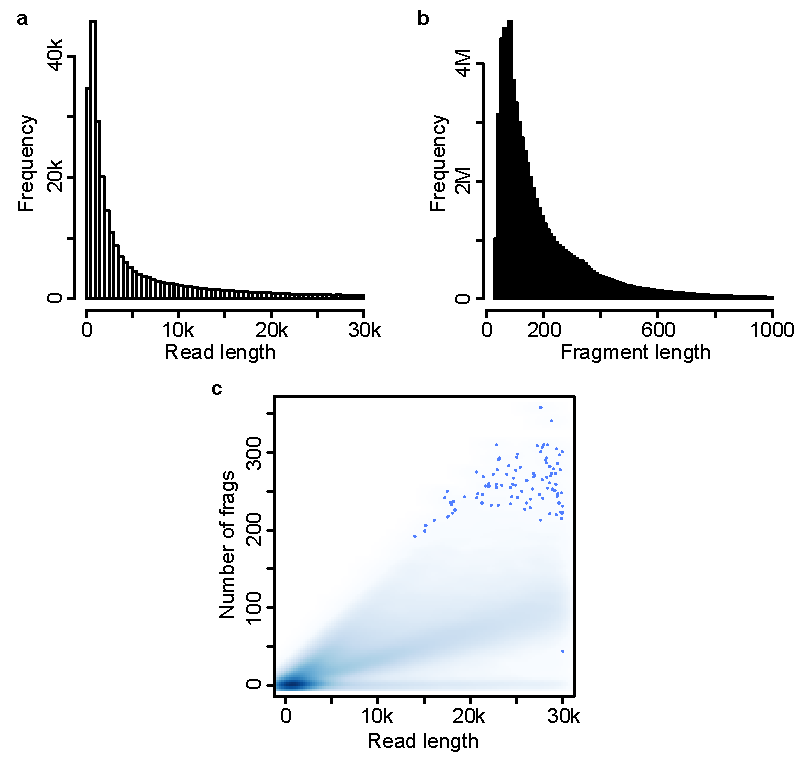
\includegraphics{read_frag_dist.pdf}
\caption{Read and fragment lengths from a SMURF-seq sequencing run.
  (a) Sequenced read length distribution.
  (b) Mapped fragment length distribution.
  (c) Scatter plot of read length and the number of fragments contained
  in the read.}
\label{read_frag_dist}
\end{figure}

%% Diploid genome
We sequenced a normal diploid female genome with SMURF-seq, resulting in
270.8k reads (mean read length of 6.75 kb) in a single run. These reads
were split into 7.28 million fragments (26.87 mean fragments per read;
Fig.~\ref{read_frag_dist}).
A CNV profile for this normal diploid genome, with the expected
(approximately flat) appearance can be seen in Fig.~\ref{cnv}a.
% Replicate
A replicate of this experiment resulted in 497.9k reads (mean read
length of 3.7 kb), which were split into 7.55 million fragments (15.16
mean fragments per read).

%% Rapid kit
The Rapid sequencing kit form Oxford Nanopore Technologies offers an
extremely fast (10 minute) and simple (2 step) protocol for library
preparation. We verified that the SMURF-seq procedure behaves similarly
using the Rapid Sequencing Kit. The 213.38k sequenced reads had a mean
read length of 3.9 kb, and were split into 2.81 million fragments.

%% skbr3 genome
Next we applied SMURF-seq to the breast cancer line SK-BR-3, generating
147.0k reads with mean length of 7.62 kb, which were split into 4.52
million fragments (30.78 mean fragments per read). We then obtained a
CNV profile using 5,000 bins, corresponding to an average bin size of
approximately 600 kb (Fig.~\ref{cnv}b).

\begin{figure}[b!]
\centering
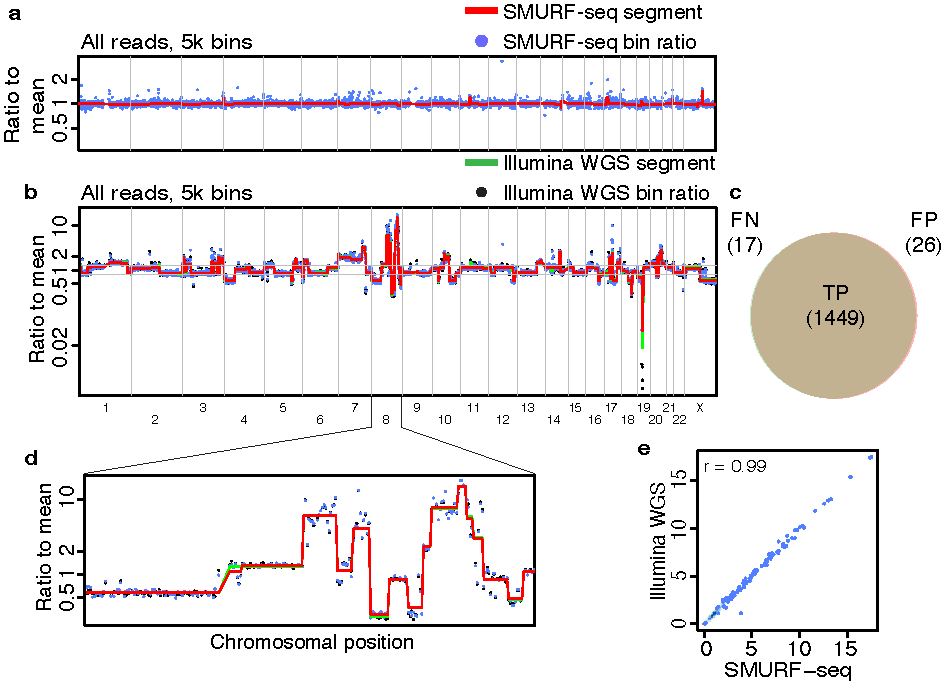
\includegraphics{ch3_fig4.pdf}
\caption{Accurate copy number profiles with SMURF-seq.
  (a) CNV profile of a normal diploid genome. Each blue point is a
  bin ratio to mean and the red line is the segmented bin ratio.
  (b) Superimposed CNV profiles of SK-BR-3 genome generated using
  SMURF-seq and Illumina WGS reads.
  (c) Venn diagram illustrating the accuracy of event calls using
  SMURF-seq compared with Illumina WGS.
  (d) Zoom-in of copy number changes on chromosome 8.
  (e) Scatter plot of bin ratio of SK-BR-3 genome using
  SMURF-seq and Illumina WGS reads. Pearson correlation of the data
  is shown.}
\label{cnv}
\end{figure}

To provide a quantification of accuracy in terms of individual CNV
events we conducted whole-genome sequencing (WGS) on the same SK-BR-3
using Illumina (5.56 million reads; 130 bp, single-end).  We used this
to define a ground truth by calling CNV events for each of the
pre-defined bins (both amplifications and deletions) based on segmented
signal with a cutoff of 1.25/0.8 (Fig.~\ref{cnv}b)
\citep{dago2014rapid,berry2017potential}. This resulted in 1,466 events
(886 amplifications, 580 deletions) from 4,953 bins. We then called
events using the identical procedure with SMURF-seq data from the same
SK-BR-3 sample. The precision and recall for SMURF-seq relative to the
Illumina calls was 0.982 and 0.988, respectively (Fig.~\ref{cnv}c).
Fig.~\ref{cnv}d shows a zoom-in of a region with extreme copy number
alterations. The bin ratios for the Illumina WGS and the SMURF-seq
profiles are highly correlated (Pearson $r$ = 0.99; Fig.~\ref{cnv}e).
% replicate
A replicate of this experiment resulted 132.64k reads (mean read length
of 7.3 kb), which were split into 4.02 million fragments (30.31 mean
fragments per read).

\begin{figure}[t!]
\centering
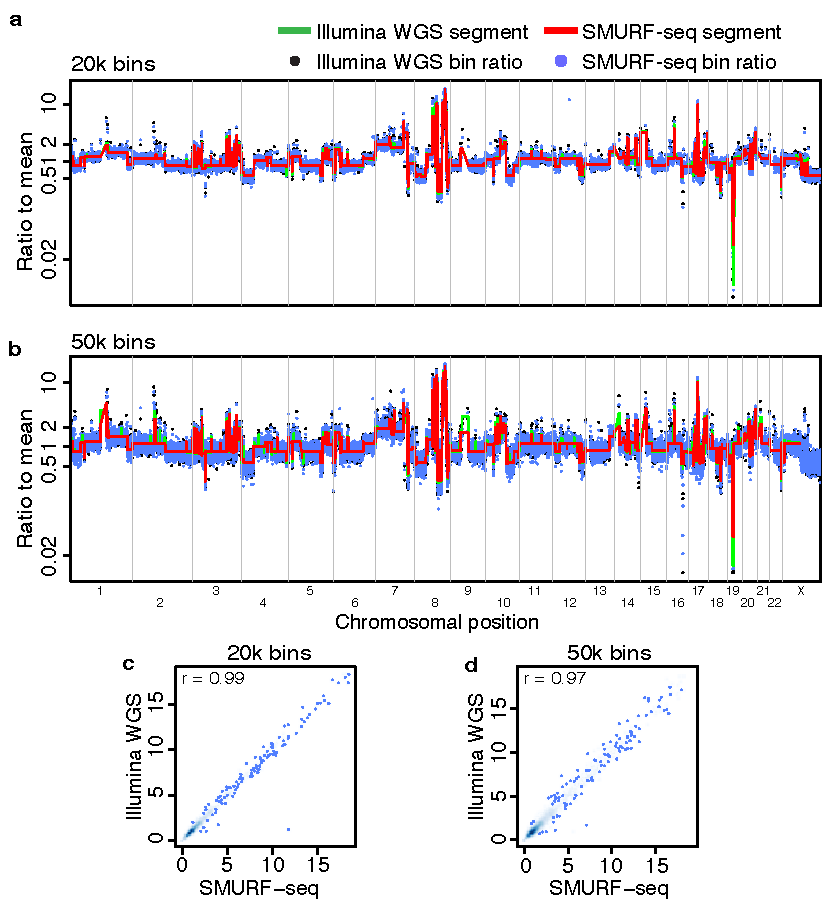
\includegraphics{skbr3_hi_res.pdf}
\caption{
  High resolution CNV profile generated using SMURF-seq is highly concordant
  with the profile generated with Illumina WGS.
  (a, b) Superimposed CNV profiles of SK-BR-3 genome generated using SMURF-seq
  and Illumina WGS at 20,000 and 50,000 bin resolutions.
  (c, d) Scatter plot of bin ratios of SK-BR-3 genome using
  SMURF-seq and Illumina WGS reads at 20,000 and 50,000 bin resolutions. }
  \label{skbr3_hi_res}
\end{figure}

%% Hige resolution profiles
We also generated higher-resolution CNV profiles at 20,000 and 50,000
bins, corresponding to an average of approximately 150 kb and 60 kb in
length respectively (Fig.~\ref{skbr3_hi_res}a, b). The profiles obtained
at these resolutions have a high correlation with the profiles obtained
using Illumina WGS (Pearson $r>$ 0.97; Fig.~\ref{skbr3_hi_res}c, d).



\subsection{Concordant profiles from fewer countable fragments}
\begin{figure}[t!]
\centering
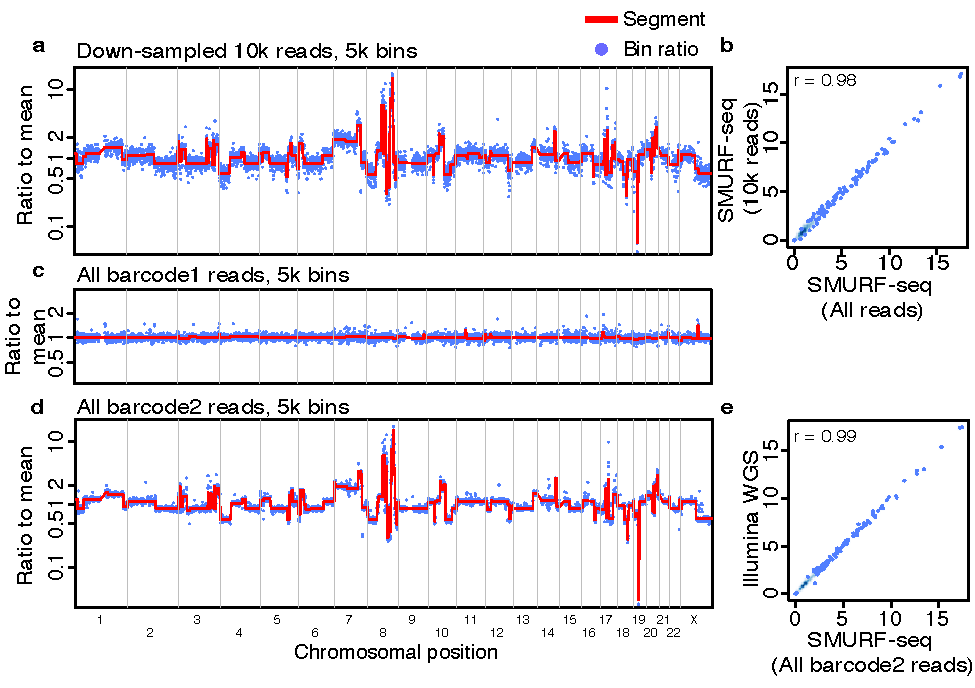
\includegraphics{ch3_fig5.pdf}
\caption{Multiple SMURF-seq CNV profiles by multiplexing in a single run.
  (a) CNV profile of SK-BR-3 genome with down-sampled 10k SMURF-seq reads.
  (b) Scatter plot of normalized bin counts of the original SMURF-seq
  data and data down-sampled to 10k SMURF-seq reads. Pearson
  correlation of the data is shown.
  (c) CNV profile of barcode01 (Normal diploid genome) reads.
  (d) CNV profile of barcode02 (SK-BR-3 cancer genome) reads.
  (e) Scatter plot of bin ratios of SK-BR-3 genome using
  multiplexed SMURF-seq and Illumina WGS reads.}
\label{cnv_mux}
\end{figure}

Several cancer-related studies have employed CNV profiling based on
low-coverage WGS \citep{macintyre2018copy,kader2016copy}.  It has
previously been demonstrated that 250k reads are sufficient for accurate
genome-wide CNV profiling of single cells \citep{baslan2015optimizing}.
At the same time, the CNV profiles from a population of cells has been
shown to have a high correlation with single-cell profiles
\citep{navin2011tumour,baslan2015optimizing}. We reasoned that using 250k
fragments for CNV profiling using a population of cells would give
useful profiles if they remained sufficiently accurate.  By
down-sampling our SMURF-seq data, we verified that 10k reads,
approximately 250k fragments, result in highly-correlated CNV profiles
(Pearson $r$ = 0.98; Fig.~\ref{cnv_mux}a, b).

Given the total capacity of the MinION instrument, this indicates that
multiple samples can effectively be barcoded and multiplexed in a single
sequencing run.
%%
To verify this we sequenced two DNA samples (normal diploid female and
SK-BR-3) in a single run.  These samples were processed with SMURF-seq
protocol and then barcoded following the standard library construction.
After demultiplexing and mapping the reads, the diploid genome had a CNV
profile as expected (Fig.~\ref{cnv_mux}c) and the SK-BR-3 CNV profile
was nearly identical to the profile obtained using Illumina WGS (Pearson
$r$ = 0.99; Fig.~\ref{cnv_mux}d, e). All the sequencing runs and the
availability of sequence data is summarized in Appendix~\ref{appendB}.

\begin{figure}[t!]
\centering
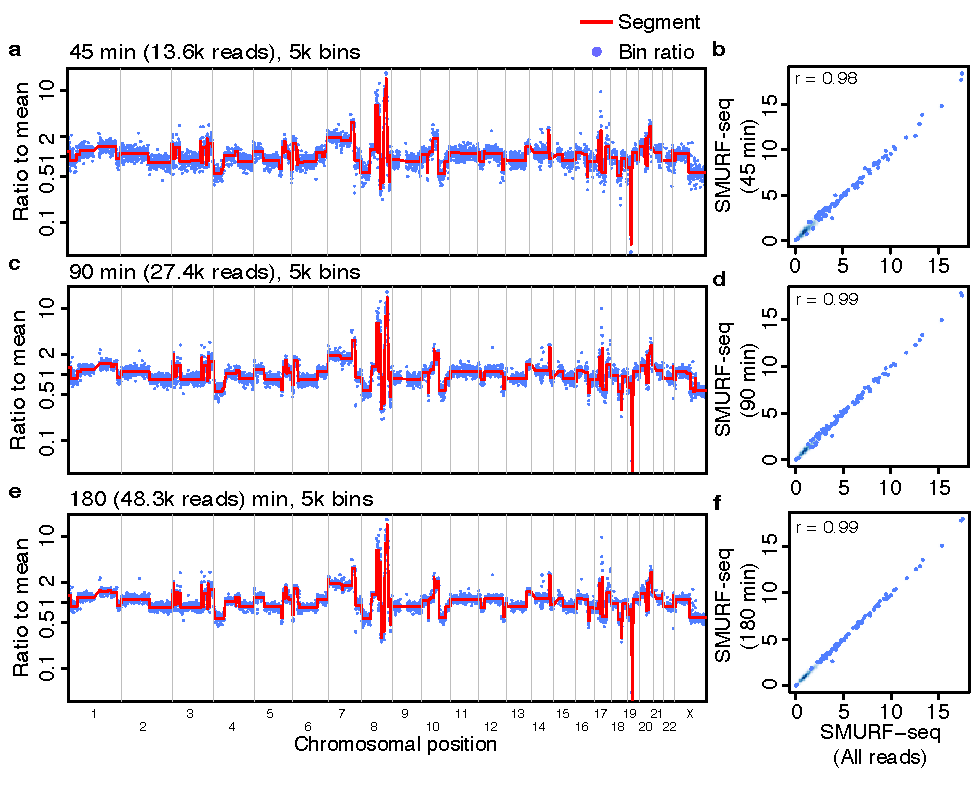
\includegraphics{cnv_time.pdf}
\caption{CNV profile with reads obtained in first few minutes of sequencing.
  (a, c, e) CNV profile  with reads obtained in the first 45, 90,
  and 180 minutes of sequencing.
  (b, d, f) Scatter plot of bin ratios of the original
  SMURF-seq data and data obtained in first 45, 90, and 180
  minutes of sequencing.}
  \label{cnv_time}
\end{figure}

%% Terminating sequencing early
Further, we verified that the CNV profile with reads generated in the
first 45, 90, and 180 minutes of starting a sequencing run had a high
correlation to the profile with reads from the complete run (Pearson $r>$
0.98; Fig.~\ref{cnv_time}).

In summary, our results demonstrate that SMURF-seq can generate more
information for CNV analysis in a single run of the Oxford MinION
sequencer, compared with either producing long reads in the usual way or
direct short-read sequencing on the same instrument.  This increased
information is in the form of increased numbers of distinct DNA
fragments sequenced, and can be leveraged in multiple ways. Applying
SMURF-seq on a single sample for a full run corresponds to higher counts
for downstream analysis. In CNV analysis, increased counts either add
confidence for a fixed resolution, or can allow higher resolution
analysis (i.e. smaller bins) at the same level of confidence.
Alternatively, the increased information throughput can effectively
reduce the time required to produce the same number of counts for CNV
analysis by terminating the sequencing earlier. Finally, the increased
information yield can be directed towards reducing the cost of
generating CNV profiles by allowing a greater degree of multiplexing.
For CNV analysis at resolutions permitted by 250k mapped fragments, our
results show SMURF-seq allows roughly 20 and up to 30 samples in a
single run, compared with 10 per run directly using short-read
sequencing.

%%%%%%%%%%%%%%%%%%%%%%%%%%%%%%%%%%%%%%%%%%%%%%%%%%%%%%%%%%%%%%%%%%%%%%%%
%%%%%%%%%%%%%%%%%%%%%%%%%%%%%%%%%%%%%%%%%%%%%%%%%%%%%%%%%%%%%%%%%%%%%%%%
%%%%%%%%%%%%%%%%%%%%%%%%%%%%%%%%%%%%%%%%%%%%%%%%%%%%%%%%%%%%%%%%%%%%%%%%
\section{Future of SMURF-seq}


%% Fragmnet identification problem
%%%%%%%%%%%%%%%%%%%%%%%%%%%%%%%%%%%%%%%%%%%%%%%%%%%%%%%%%%%%%%%%%%%%%%%%
%%%%%                                                              %%%%%
%%%%% Chapter 4: Identifying SMURF-seq fragment boundaries         %%%%%
%%%%%                                                              %%%%%
%%%%%%%%%%%%%%%%%%%%%%%%%%%%%%%%%%%%%%%%%%%%%%%%%%%%%%%%%%%%%%%%%%%%%%%%

\chapter{Identifying fragment boundaries on a SMURF-seq read}
\label{ch4}

%%%%%%%%%%%%%%%%%%%%%%%%%%%%%%%%%%%%%%%%%%%%%%%%%%%%%%%%%%%%%%%%%%%%%%%%
%%%%%%%%%%%%%%%%%%%%%%%%%%%%%%%%%%%%%%%%%%%%%%%%%%%%%%%%%%%%%%%%%%%%%%%%
%%%%%%%%%%%%%%%%%%%%%%%%%%%%%%%%%%%%%%%%%%%%%%%%%%%%%%%%%%%%%%%%%%%%%%%%
\section{Motivation}
%% Sequencing tech and mapping methods
New sequencing methods motivate development of new algorithms for
mapping and analysis of sequences generated using these methods. A few
significant developments include BLAST \cite{altschul1990basic} and
FASTA \cite{pearson1988improved} motivated by database searches with the
advent of Sanger sequencing, BWA \cite{li2009fast} and Bowtie
\cite{langmead2009ultrafast} inspired by high-throughput short-read
sequencing, and BLASR \cite{chaisson2012mapping} by single-molecule
long-read sequencing.
%% SMURF-seq
SMURF-seq has enabled efficient short-read sequencing for read-counting
applications on portable long-read machines.  However, efficient methods
tailored for mapping SMURF-seq reads are still lacking; Especially as
SMURF-seq protocol evolves and the fragments become shorter, and thus,
making the mapping process challenging in terms of identifying accurate
fragment locations and boundaries.

%% current SMURF-seq
As currently implemented, SMURF-seq protocol uses a single restriction
enzyme (SaqAI) to fragment DNA molecules to $\sim$150 bp. However,
depending on the downstream application, the fragment lengths need to be
just long enough to ensure unique mappability to a sufficient fraction
of the genome.
%% making fragments shorter
Fragments could be made shorter using methods discussed in section
\ref{}.  As an example, for copy-number profiling (at low
resolutions, as used for tumor samples) the fragment lengths could be as
short as 40 bp.

%% current barriers and how to remove them
We used BWA-MEM \cite{li2013aligning} to align SMURF-seq reads generated
with the current protocol, which consists of fragments that are
typically over 100 bp. Though not designed to align SMURF-seq reads,
BWA-MEM is designed for split read alignment, and it works sufficiently
well at these fragment lengths.  SMURF-seq reads can also be aligned
with other mapping tools capable of split-read alignment such as
Minimap2 \cite{li2018minimap2} and LAST \cite{kielbasa2011adaptive}.
However, all of these tools are either designed for aligning short reads
with low sequencing error or long reads with high sequencing error.
%
Moreover, since these tools are not designed for SMURF-seq reads, they
lack certain capabilities; e.g. they do not provide a method to estimate
the number of fragments or determine the optimal fragment boundaries in
a SMURF-seq reads, and these become increasingly important with shorter
fragments.

%% challenges as the fragments get shorter
The significance of having accurate fragment boundaries is understood by
looking at the fraction of the genome that is uniquely mappable. For the
human reference genome (hg19), when allowing no mismatches or indels,
the fraction of the genome that is uniquely mappable reduces by 0.06\%
when going from 150 to 145 bp, whereas it reduces by 2.02\% when going
from 40bp to 35bp (Fig.~\ref{dzones}).
% how it affects SMURF-seq read
Thus, as the fragments get shorter, the probability of a fragment that
originated from a unique location on the genome to misalign to an
ambiguous location or vice-versa increases.
% reads with errors
% TODO: Improve sentence below
Further, as sequencing errors are considered the difference in unique
mappability due to having inaccurate fragment boundaries is likely to
increase.
%
Thus, as the fragments become shorter, having accurate fragment
boundaries would improve the sensitivity of aligning SMURF-seq reads.

\begin{figure}[t!]
\centering
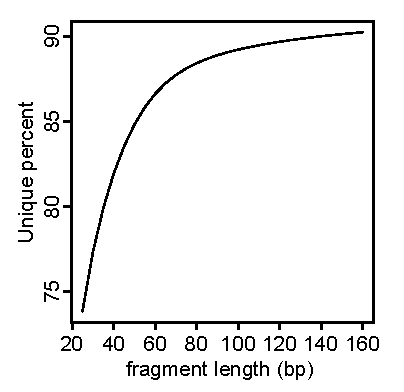
\includegraphics{ch4_fig1.pdf}
\caption{The fraction of genome that is uniquely mappable decreases with
          fragment length.}
\label{dzones}
\end{figure}


%% How will our method remove the current barrier
We propose a method to estimate the number of fragments on a SMURF-seq
read. We define a score function for aligning a SMURF-seq read, study
the distribution of aligning reads and reference generated at random,
and estimate the number of fragments in a SMURF-seq read by comparing
its alignment score with the distribution of aligning random reads for
all possible fragmentations of a read. Then we show the accuracy of our
method using from simulated genomes and SMURF-seq reads. Further, we
empirically show that this method could also be used with a general
score function.

%%%%% How will this improve scientific capacity and knowledge




%%%%%%%%%%%%%%%%%%%%%%%%%%%%%%%%%%%%%%%%%%%%%%%%%%%%%%%%%%%%%%%%%%%%%%%%
%%%%%%%%%%%%%%%%%%%%%%%%%%%%%%%%%%%%%%%%%%%%%%%%%%%%%%%%%%%%%%%%%%%%%%%%
%%%%%%%%%%%%%%%%%%%%%%%%%%%%%%%%%%%%%%%%%%%%%%%%%%%%%%%%%%%%%%%%%%%%%%%%
\section{Background}
\label{ch4_background}
In the early days of DNA sequencing, as the number of nucleotides
sequenced grew, comparison of DNA sequences became an indispensable tool
to a biologist.
%
DNA sequence comparison can be broadly classified into global alignment
\cite{needleman1970general} and local alignment
\cite{smith1981identification}. A global alignment seeks an optimal
alignment between two sequences such that each base of one sequence is
aligned to each base of the other sequences. On the other hand, a local
alignment seeks an optimal alignment between any subsequences of the
sequences being compared.

Comparison of two sequences, even unrelated or random sequences, always
produces an optimal alignment. This motivated the development of
approaches to differentiate a ``meaningful'' alignment from alignment of
unrelated sequences. These methods determine the significance of an
alignment by comparing the alignment score with a null distribution of
alignment scores of unrelated sequences. Determining the appropriate null
distribution was the subject of an enormous amount of research, some of
which are summarized below.

%% Simulation studies
In the context of local alignment, at the time of the initial studies on
the score distribution of unrelated sequences, mathematical tools to
understand the null distributions were still lacking, and these studies
relied on empirical distributions generated from aligning unrelated
sequences.
%%
In \cite{smith1985statistical}, it is shown that the similarity score is
proportional to the logarithm of the length of the sequences being
compared, and the standard deviation is independent of the sequence
length. The significance of an alignment was determined from the number
of standard deviations over mean of the alignment score.
%% Dependence on sequence properties
These studies \cite{lipman1984statistical} also highlight that the
statistical properties \cite{smith1983statistical}, such as nucleotide
frequencies or codon usage, of the sequences affect the distribution of
the alignment scores.  Generating a null distribution from an incorrect
model could lead to an alignment of unrelated sequences being dubiously
declared significant. Several methods are available to generate random
sequences preserving these statistical properties
\cite{fitch1983random,altschul1985significance}.

%% Mike's approach: coin tossing
Erdos and Renyi \cite{erdos1975length} presented results for the length
of the longest headrun in a the first $n$ tosses of a biased coin.  The
length of the longest headrun in coin tosses is equivalent to the number
of matches between two DNA sequences when shifts in the starting and
ending positions of the sequences are not allowed, with the probability
of head equal to the probability of match between letters of the DNA
alphabet.
% coin tossing with shifts and fixed mismatches.
In \cite{arratia1985erdos}, this is generalized to matches between DNA
sequences, while allowing shifts. These results indicate that allowing
shifts doubles the length of the longest headrun. Results for the
longest headrun allowing for up to $k$ mismatches and sequences
generated from a Markov chain are also considered.
% EVD approximation
In \cite{arratia1986extreme,gordon1986extreme} the distribution of the
longest matches is shown to a have an extreme value distribution with
mean that is proportional to the logarithm of the sequences lengths and
variance independent of sequence length. Here, when considering only
matches, the asymptotic extreme value distribution is shown by
considering a maximum of geometric distributions, and when mismatches
are allowed, it is shown by considering a maximum of negative binomial
distributions.
% poisson approximation
An alternate approach is a Poisson approximation for the distribution of
the longest match \cite{arratia1989erdos}.

%% Dembo and Karlin's approach
An crucial aspect of in aligning nucleic acid and protein sequences is
using the appropriate score function. For example, PAM and Dayoff
matrices is used for protein sequences \cite{}, and xxx is used for DNA
sequences \cite{}.  The score function used alters the score of the
aligned sequences and thus the alignment score distribution of unaligned
sequences.
% Headrun approach does not consider score function
However, the approach based on the length of the headruns does not
consider the score function used for an alignment.
%
In \cite{}, it is shown that the score distribution of aligning
unrelated sequences for any score function (that has at least one
positive score and the expected score is negative) has the form of an
extreme value distribution, and and explicit formulas that its parameters
are provided.
% distribution of letters, and log-odds ratio



%% alignment allowing gaps

%% BLAST

%% Profile alignment

%% Global alignment score distribution

%% Differneces between these and the k=1 frag id problem




%% local alignment
% The local alignment score distribution has been studied extensively,
% especially in the context of BLAST score statistics
% \cite{altschul1990basic,altschul199627}.  The distribution of the local
% alignment score is well approximated by the extreme value distribution
% (EVD) \cite{karlin1990methods,
% karlin1990statistical,dembo1994limit,dembo1991strong}.

% It has also been shown that the distribution of the maximum score
% obtained when a profile sequence is aligned to all possible positions of
% a random sequence has a limiting extreme value distribution
% \cite{goldstein1994approximations}.


%%%%%%%%%%%%%%%%%%%%%%%%%%%%%%%%%%%%%%%%%%%%%%%%%%%%%%%%%%%%%%%%%%%%%%%%
%%%%%%%%%%%%%%%%%%%%%%%%%%%%%%%%%%%%%%%%%%%%%%%%%%%%%%%%%%%%%%%%%%%%%%%%
%%%%%%%%%%%%%%%%%%%%%%%%%%%%%%%%%%%%%%%%%%%%%%%%%%%%%%%%%%%%%%%%%%%%%%%%
\section{Fragment Identification problem}
%% string properties
Let $\Sigma$ be an alphabet. A string $X$ is a sequence of letters $a_0
a_1 \dots a_{n-1}$, where $a_i \in \Sigma$; $|X|$ denotes the length of
the string $X$; and $X[i \dots j] = a_i \dots a_{j-1}$ is a substring of
$X$.

%% reference string
The reference string $T$ is generated from the DNA alphabet $\Sigma =
\{A, T, G, C\}$, with $|T| = n$.
%% SMURF-seq string
A SMURF-seq read $S$ is generated by concatenating substrings (called
fragments) of $T$, with no information available \textit{a priori} about
the number, length, orientation (forward or reverse-complement), and the
position on $T$ of these fragments.  Further, $S$ contains sequencing
errors with a rate $\rho$. Let $|S| = m$ and $m \ll n$.

%% fragment set
A fragment set $P$ is an set of start locations of fragments on $S$. $P
\subset \{0 \dots m-1\}$ and $|P| = k$, with the rule that $0$ is in $P$
always.
%%
By convention we consider the set $P$ to be ordered such that if $i < j$
then $P_i < P_j$.
%%
For a fragment set $P$, $\sum_{i = 1}^{k} P_{i+1} - P_i = m$ and we say
that the $i^{\text{th}}$ of $S$ is the substring $S[P_i \dots P_{i+1}]$,
with $P_{k+1} = m$.

%% fragment identification problem
For a given $T$ and $S$, the fragment identification problem is to
determine the elements of the fragment set $P$ such that it corresponds
to the start locations of fragments contained in $S$.



%%%%%%%%%%%%%%%%%%%%%%%%%%%%%%%%%%%%%%%%%%%%%%%%%%%%%%%%%%%%%%%%%%%%%%%%
%%%%%%%%%%%%%%%%%%%%%%%%%%%%%%%%%%%%%%%%%%%%%%%%%%%%%%%%%%%%%%%%%%%%%%%%
%%%%%%%%%%%%%%%%%%%%%%%%%%%%%%%%%%%%%%%%%%%%%%%%%%%%%%%%%%%%%%%%%%%%%%%%
\section{Approach to the fragment identification problem}
We approach the fragment identification problem by defining a score
function as follows:
%% score function
For a given fragment set $P$, we define the score of aligning $S$ to $T$
as: \[score_T(S,P) = \sum_{i=1}^{k} \max\{score(T[u \dots v], S[P_i
\dots P_{i+1}]): 0 \leq u < v \leq n\}.\]
%
This allows us to consider the fragment identification problem as two
inter-related problems: (1) Determining $k$, the size of the fragment
set, and (2) given $k$, determining the elements of $P$ such that
$score_T(S, P)$ is maximized.

%% Any k gives a score. Highest score does not correspond to the opt.
By the score function defined above, to determine the elements of the
fragment set $P$, requires the knowledge of the number of fragments $k$
and this is not known \textit{a priori}. Further, the $k$ that maximizes
the score function would almost never correspond to the optimal fragment
set. As an example, taking $k=m-1$ which corresponds to taking each base
as a fragment would maximize the score, however, this is a non-sensical
alignment.

%% Outline of our statistical approach.
We propose to estimate the number of fragments $k$ by aligning a read
to the reference genome with different $k$. For each of these
fragmentations, we determine the p-value by comparing the alignment
score with the null distribution generated from aligning reads generated
at random to a reference genome generated at random. Finally, we choose
the fragmentation with lowest p-value as the optimal fragmentation.

%% Differences with the local alignment approach We are interested in
%% opt frags, and not significant alignment
The fragment identification problem differs from the alignment problems
described in section \ref{ch4_background} in a crucial manner. For the
fragment identification problem we have the reference genome, and it is
assumed that the reads always arise from this genome; the score
distribution of sequences generated at random is used to determine the
optimal number of fragments on a SMURF-seq read. Whereas in the context
of local alignment the score distribution of aligning random reads are
used to determine a ``meaningful'' alignment by comparing the alignment
score of sequences with the random null distribution.


%%%%%%%%%%%%%%%%%%%%%%%%%%%%%%%%%%%%%%%%%%%%%%%%%%%%%%%%%%%%%%%%%%%%%%%%
%%%%%%%%%%%%%%%%%%%%%%%%%%%%%%%%%%%%%%%%%%%%%%%%%%%%%%%%%%%%%%%%%%%%%%%%
%%%%%%%%%%%%%%%%%%%%%%%%%%%%%%%%%%%%%%%%%%%%%%%%%%%%%%%%%%%%%%%%%%%%%%%%
\section{Score distribution under a random model}
\paragraph{Problem definition for a random model:}
The strings $T$ and $S$ are generated by drawing letters independently
from the same distribution from an alphabet $a \in \Sigma$ with
probability $p_a$ such that $\sum_{a \in \Sigma} p_a = 1$.  For a given
fragment set $P$ containing $k$ elements, we need to determine the
distribution of $score_T(S, P)$. First, we consider the score
distribution when $k = 1$, i.e. the entire read aligns as one fragment.
Then we consider the score distribution when $k > 1$.

%% Score function
We use the following score function to obtain the distribution of
$score_T(S,k)$:
\begin{equation*}
\label{exact_score}
score(a,b)=\begin{cases} 1 & \text{if } a = b \\
            0 & \text{if } a\neq b \\
            -\infty & \text{otherwise.}
\end{cases}
\end{equation*}

\subsection{Score distribution of one fragment}
%% How fragment identification problem differs from these
The distribution of $score_T(S,1)$ differs from the local alignment as
we require an end-to-end alignment of $S$ to a substring of $T$. It also
differs from the profile score distribution since the letters of $S$ are
generated at random.

%% distribution for k = 1
Based on these results, the distribution of $score_T(S,1)$ is likely to
follow an extreme value distribution. The heuristic is as follows.
% heuristic of proof
Let $X_j$ denote the score of aligning $S$ with $T[j \dots j+m-1]$, then
\[X_j = \sum_{i=0}^{m-1} score(S[i],T[j+i]), j = 0, \dots, n-m+1.\]
Since the letters of T and S are iid, we have \[X_j \sim binom(m,p)\]
where $p = \sum_{a=\Sigma} p_a^2$.  For a large enough $m$, $X_j$ can
be approximated by a normal distribution as \[X_j \sim N(mp, mp(1-p)).
\] $score_T(S,1)$ is the maximum score over all positions in $T$,
\[score_T(S,1) = \max_{0 \leq j \leq n-m+1} X_j.\] $score_T(S,1)$ is a
maximum of normal distributions, which follows an extreme value
distribution \cite{kotz2000extreme}.
%% m-dependence
Here, we have a dependence between $X_j$ and $X_k$ for $|j - k| < m$.

%% distribution and qq plot

%% Distribution as a function of fragment length

%% Distribution as a function of genome length

\subsection{Score distribution for a given fragment set}



%%%%%%%%%%%%%%%%%%%%%%%%%%%%%%%%%%%%%%%%%%%%%%%%%%%%%%%%%%%%%%%%%%%%%%%%
%%%%%%%%%%%%%%%%%%%%%%%%%%%%%%%%%%%%%%%%%%%%%%%%%%%%%%%%%%%%%%%%%%%%%%%%
%%%%%%%%%%%%%%%%%%%%%%%%%%%%%%%%%%%%%%%%%%%%%%%%%%%%%%%%%%%%%%%%%%%%%%%%
\section{Identifying optimal fragment boundaries}



%%%%%%%%%%%%%%%%%%%%%%%%%%%%%%%%%%%%%%%%%%%%%%%%%%%%%%%%%%%%%%%%%%%%%%%%
%%%%%%%%%%%%%%%%%%%%%%%%%%%%%%%%%%%%%%%%%%%%%%%%%%%%%%%%%%%%%%%%%%%%%%%%
%%%%%%%%%%%%%%%%%%%%%%%%%%%%%%%%%%%%%%%%%%%%%%%%%%%%%%%%%%%%%%%%%%%%%%%%
\section{Estimating the number of fragments}




%%%%%%%%%%%%%%%%%%%%%%%%%%%%%%%%%%%%%%%%%%%%%%%%%%%%%%%%%%%%%%%%%%%%%%%%
%%%%%%%%%%%%%%%%%%%%%%%%%%%%%%%%%%%%%%%%%%%%%%%%%%%%%%%%%%%%%%%%%%%%%%%%
%%%%%%%%%%%%%%%%%%%%%%%%%%%%%%%%%%%%%%%%%%%%%%%%%%%%%%%%%%%%%%%%%%%%%%%%
\section{Results}


\subsection{Exact matching reads}

\subsection{Reads with mismatches}


%% Conclusion
%%%%%%%%%%%%%%%%%%%%%%%%%%%%%%%%%%%%%%%%%%%%%%%%%%%%%%%%%%%%%%%%%%%%%%%%
%%%%%                                                              %%%%%
%%%%% Chapter 5: Conclusions                                       %%%%%
%%%%%                                                              %%%%%
%%%%%%%%%%%%%%%%%%%%%%%%%%%%%%%%%%%%%%%%%%%%%%%%%%%%%%%%%%%%%%%%%%%%%%%%
\chapter{Conclusions}
\label{ch5}


\singlespacing

%%%%%%%%%%%%%%%%%%%%%%%%%%%%%%%%%%%%%%%%%%%%%%%%%%%%%%%%%%%%%%%%%%%%%%%%
%%%%%%%%%%%%%%%%%%%%%%%%%%%%%%%%%%%%%%%%%%%%%%%%%%%%%%%%%%%%%%%%%%%%%%%%
%%%%%%%%%%%%%%%%%%%%%%%%%%%%%%%%%%%%%%%%%%%%%%%%%%%%%%%%%%%%%%%%%%%%%%%%
\newpage
\bibliographystyle{unsrt}
\bibliography{thesis}

%%%%%%%%%%%%%%%%%%%%%%%%%%%%%%%%%%%%%%%%%%%%%%%%%%%%%%%%%%%%%%%%%%%%%%%%
%%%%%%%%%%%%%%%%%%%%%%%%%%%%%%%%%%%%%%%%%%%%%%%%%%%%%%%%%%%%%%%%%%%%%%%%
%%%%%%%%%%%%%%%%%%%%%%%%%%%%%%%%%%%%%%%%%%%%%%%%%%%%%%%%%%%%%%%%%%%%%%%%
\begin{appendices}
\doublespacing
  %%%%%%%%%%%%%%%%%%%%%%%%%%%%%%%%%%%%%%%%%%%%%%%%%%%%%%%%%%%%%%%%%%%%%%%%
%%%%%                                                              %%%%%
%%%%% Appendix A: Detailed SMURF-seq protocol                      %%%%%
%%%%%                                                              %%%%%
%%%%%%%%%%%%%%%%%%%%%%%%%%%%%%%%%%%%%%%%%%%%%%%%%%%%%%%%%%%%%%%%%%%%%%%%
\chapter{Supplemental methods}
\label{appendA}

\section*{DNA samples}
The normal diploid female DNA was purchased from Promega (Cat. no.
G1521).  Breast cancer cell line SK-BR-3 (American Type of Culture
Collection (ATCC), Cat. no. HTB-30) was cultured in RPMI-1640 medium
(Thermo Fisher Scientific, Cat. no. 11875093) supplemented with 10\%
fetal bovine serum (FBS) (Thermo Fisher Scientific, Cat. no. 35011CV)
and was maintained at \SI{37}{\degree} in a humidified chamber supplied
with 5\% $\text{CO}_2$ and was regularly tested for mycoplasma
infection.

\section*{Cell lysis and DNA purification}
The DNA from SK-BR-3 cells was extracted and purified with the QIAamp
DNA Blood Mini Kit (Qiagen, Cat. no. 51104) following the protocol for
cultured cells given by the manufacturer. RNA and proteins in the cells
were degraded using RNase A stock solution
(\SI{100}{\milli\gram}/\SI{}{\milli\litre}) (Qiagen, Cat.  no. 19101)
and Protease-K (Qiagen, Cat. no. 19133) respectively. Both purchased
female diploid DNA and extracted SK-BR-3 DNA were treated with the same
downstream processes.

\section*{Fragmenting genomic DNA}
2-\SI{3}{\micro\gram} of genomic DNA was fragmented with restriction
enzyme Anza 64 SaqAI (Thermo Fisher Scientific, Cat. no. IVGN0644) for
\SI{30}{\minute} at \SI{37}{\degree}. The fragmented DNA was cleaned
with the QIAquick PCR purification kit (Qiagen, Cat. no. 8106) and
eluted with \SI{34}{\micro\litre} nuclease-free water. The concentration
of DNA was quantified on a Qubit Fluorometer v3 (Thermo Fisher
Scientific, cat. no. Q33216) with the Qubit dsDNA HS assay kit (Thermo
Fisher Scientific, cat. no. Q32854).

\section*{Ligation of fragmented DNA}
\SI{500}{\nano\gram} of fragmented DNA in \SI{10}{\micro\litre}
nuclease-free water was mixed with \SI{10}{\micro\litre} Anza T4 DNA
Ligase Master Mix (Thermo Fisher Scientific, Cat. no. IVGN210-4) and
incubated for \SI{30}{\minute} at room temperature. The ligated DNA was
cleaned with 2\(\times\) volume Ampure XP beads (Beckman Coulter, Cat.
no. A63881) and eluted in nuclease-free water. This step was done in
multiple tubes if more than \SI{500}{\nano\gram} of fragmented DNA was
needed to be ligated. The concentration of DNA was quantified on a Qubit
Fluorometer v3 with the Qubit dsDNA HS assay kit to ensure
\(\geq\)\SI{1}{\micro\gram} (\(\geq\) \SI{400}{\nano\gram}, if the Rapid
kit was used for library preparation) remained. The size of the ligated
DNA molecules were assessed with \(1\%\) agarose gel electrophoresis run
at \SI{90}{\volt} for \SI{30}{\minute}.

\section*{Library preparation (SQK-LSK108 1D DNA by ligation)}
\SI{1}{\micro\gram} of re-ligated DNA in \SI{45}{\micro\litre} of
nuclease-free water was end-repaired and dA-tailed (New England Biolabs
(NEB), Cat. no. E7546), followed by elution in nuclease-free water after
\(1.5\times\) volume Ampure XP beads clean-up. Sequencing adapters
(AMX1D) were ligated with Blunt/TA Ligase Master Mix (NEB, Cat.no.
M0367) and cleaned with \(0.4\times\) volume Ampure XP beads and eluted
using \SI{15}{\micro\litre} Elution Buffer (ELB) following the
manufacturer's protocol (Oxford Nanopore Technologies (ONT), 1D genomic
DNA by ligation protocol).

\section*{Multiplexed library preparation (EXP-NBD103 and SQK-LSK108)}
\SI{700}{\nano\gram} of each re-ligated sample in \SI{45}{\micro\litre}
of nuclease-free water was end-repaired, dA-tailed (NEB, Cat. no.
E7546), cleaned with \(1.5\times\) volume Ampure XP beads and eluted in
nuclease-free water. Different Native Barcodes (NB-x) for each sample
was ligated with Blunt/TA Ligase Master Mix (NEB, Cat.no. M0367),
cleaned with \(2\times\) volume Ampure XP beads and eluted in
nuclease-free water. Equimolar amounts of each sample was pooled to have
\SI{700}{\nano\gram} of DNA in \SI{50}{\micro\litre} water. Barcode
adapters (BAM) were ligated with Quick T4 DNA Ligase (NEB, Cat. no.
E6056), cleaned with \(0.4\times\) volume Ampure XP beads and eluted
using \SI{15}{\micro\litre} Elution Buffer (ELB) following the
manufacturer's protocol (ONT, 1D native barcoding genomic DNA).

\section*{Library preparation (SQK-RAD003 Rapid sequencing)}
\SI{400}{\nano\gram} of re-ligated DNA was concentrated with \(2\times\)
volume Ampure XP beads to \SI{7.5}{\micro\litre} nuclease-free water.
DNA was tagmented with Fragmentation Mix (FRA), and Rapid 1D Adapter
(RPD) was attached following the manufacturer's protocol (ONT, rapid
sequencing).

\section*{MinION sequencing and base-calling}
All the prepared libraries were loaded on R9.5 Flowcells following the
manufacturer's protocol (ONT) and sequenced for up to 48 hours using the
script specific to library preparation protocol. Base-calling and
de-multiplexing barcoded reads were performed using ONT Guppy (2.3.5)
with the appropriate parameters based on the library preparation kit.

\section*{Sequencing RE digested normal diploid genome}
% RE digestion
\SI{1}{\micro\gram} of genomic DNA was fragmented with restriction
enzyme Anza 64 SaqAI (Thermo Fisher Scientific, Cat. no. IVGN0644) for
\SI{30}{\minute} at \SI{37}{\degree}. The fragmented DNA was cleaned
with the QIAquick PCR purification kit (Qiagen, Cat. no. 8106) and
eluted with \SI{31}{\micro\litre} nuclease-free water. The concentration
of DNA was quantified on a Qubit Fluorometer v3 (Thermo Fisher
Scientific, cat. no. Q33216) with the Qubit dsDNA HS assay kit (Thermo
Fisher Scientific, cat. no. Q32854).

% 1D library prep.
\SI{0.5}{\micro\gram} of restriction enzyme digested DNA in
\SI{45}{\micro\litre} of nuclease-free water was end-repaired and
dA-tailed (New England Biolabs (NEB), Cat. no. E7546), followed by
elution in nuclease-free water after \(1.5\times\) volume Ampure XP
beads clean-up. Sequencing adapters (AMX1D) were ligated with Blunt/TA
Ligase Master Mix (NEB, Cat.no. M0367) and cleaned with \(1.0\times\)
volume Ampure XP beads (manufacturer's protocol uses \(0.4\times\)
volume XP beads, we increased to \(1.0\times\) to get as many short
molecules as possible) and eluted using \SI{15}{\micro\litre} Elution
Buffer (ELB) following the manufacturer's protocol (Oxford Nanopore
Technologies (ONT), 1D genomic DNA by ligation protocol).

% MinION sequencing and base-calleing
The prepared library was loaded on R9.4 Flowcell following the
manufacturer's protocol (ONT) and sequenced for 48 hours.  Base-calling
was performed using ONT Guppy (2.3.5).

\section*{Estimation of copy number variations}
CNV profiles were generated using the procedure described in
\citep{baslan2012genome,kendall2014computational} with the modification
employed in \citep{gerdtsson2018multiplex,malihi2018clonal}.  Briefly,
the human reference genome (hg19) was split into 5,000 (20,000 or
50,000) bins containing an equal number of uniquely mappable locations
and the bin counts were determined using uniquely mapped fragments.
Bins with spuriously high counts (`bad bins', typically around
centromeric and telomeric regions) were masked for downstream analysis
\citep{kendall2014computational}.  This procedure normalizes bin counts
for biases correlated with GC content by fitting a LOWESS curve to the
GC content by bin count, and subtracting the LOWESS estimate from each
bin \citep{kendall2014computational}.  Circular binary segmentation
(CBS) \citep{olshen2004circular}, implemented in DNAcopy
\citep{seshan2010dnacopy} package, then identifies breakpoints in the
normalized bin counts.  Following
\citep{gerdtsson2018multiplex,malihi2018clonal}, after CBS, spurious
segmentation calls were removed.  The influence of the GC content
correction can be seen in Additional file 1: Figure~S14.

\section*{Comparison with Illumina WGS of SK-BR-3 genome.}
DNA from SK-BR-3 cells was used to construct WGS library with the
NEBNext UltraII FS DNA Library Prep Kit (NEB, Cat. no. E7805) following
the manufacturer's instructions. After library quality and quantity
assessment with Qubit 3.0 HS dsDNA assay and BioAnalyzer HS dsDNA assay
(Agilent), libraries were sequenced on HiSeq 2500 (Illumina) with
single-end 130 cycles mode.

The reads were mapped with BWA-MEM using the default parameters, PCR
duplicates were removed, and CNV profiles were generated using exactly
the same method as used for SMURF-seq reads.  The scatter plots and
Pearson correlations comparing the CNV profiles were produced using R.

%%%%%%%%%%%%%%%%%%%%%%%%%%%%%%%%%%%%%%%%%%%%%%%%%%%%%%%%%%%%%%%%%%%%%%%%
%%%%%                                                              %%%%%
%%%%% Appendix B: Mapping SMURF-seq reads                          %%%%%
%%%%%                                                              %%%%%
%%%%%%%%%%%%%%%%%%%%%%%%%%%%%%%%%%%%%%%%%%%%%%%%%%%%%%%%%%%%%%%%%%%%%%%%
\chapter{Mapping SMURF-seq reads with long-read aligners}
\label{appendB}
\section*{Simulating SMURF-seq reads to evaluate mapping programs}
To test these mapping tools, we chose to create simulated reads with the
technical characteristics we expect in idealized SMURF-seq data. We
first selected a fragment length $\ell$ and a number $k$ of fragments
per read. Then, for a given WGS nanopore data set, we took the set of
mapped long reads as determined by BWA-MEM (with \texttt{-x ont2d}
option).
Each of the mapped reads was split into fragments of length $\ell$ (with
a random offset of $0$ to $\ell-1$ at the start of the long read). Each
fragment was validated by requiring that it did not overlap a deadzone
in the genome (as determined by the deadzone program available from
https://github.com/smithlabcode/utils for 40 bp). The reason for
excluding deadzones is that even when a short fragment has a ``known''
mapping location when it is part of a longer read, we cannot compare its
reported mapping location as a short fragment with that known location,
since we expect any good mapping algorithm to identify that the fragment
maps ambiguously. Among these validated fragments, subsets of $k$ were
sampled uniformly at random and concatenated (in random order and
orientation) to form simulated SMURF-seq reads.

The first and last fragments in a read should be slightly easier to
identify and map than the rest, since one of their boundaries is
known. Using the above procedure, we select $k=20$ so that the
simulated reads have a sufficient number of fragments to eliminate the
influence of the first and last fragments in each read on the
results. There is no need to have large $k$ otherwise.

By lowering $\ell$ and making the fragments shorter, the task of
mapping the fragments becomes more challenging. Real SMURF-seq reads
have fragment lengths determined by restriction site density, size
selection and other aspects of the experiments. But in testing mapping
algorithms and optimizing parameters, there is no disadvantage to
making the task more challenging. We only need to be able to
distinguish the relative performance of different mapping tools and
parameter combinations. Real SMURF-seq reads have varying fragment
lengths, but in evaluating mapping tools, there is no need to
randomize fragment lengths. None of the algorithms we evaluated are
capable of either deducing or leveraging the fact that all simulated
fragments have the same length. We selected $\ell = 100$, which
begins to challenge the various mapping strategies. These values of
$\ell$ are slightly lower than the average in real SMURF-seq data.


\section*{Evaluating performance using simulated SMURF-seq reads}
Within the simulated reads, the boundaries of each fragment are known
\textit{a priori}, as are their mapping locations. We used this
information to evaluate mapping tools in terms of (1) how well they
identify fragments purely for the purpose of counting molecules, which
is the primary information used in CNV analysis, and (2) how well they
identify individual mapping bases within reads. The latter criteria
becomes important in challenging cases and will be increasingly
important as fragment sizes are reduced.

Performance on identifying fragments: After mapping these simulated
reads, each mapping result is called a predicted fragment. Each
predicted fragment is considered a positive prediction, and we assume
an arbitrary order over positive predictions. A positive prediction is
a true positive if:
\begin{itemize}
\item The predicted fragment maps uniquely.
\item The mapping locations of at least half the bases in the
  predicted fragment are equal to the original mapping locations for
  those bases, and those bases are all part of the same original
  fragment (we assume that it is unlikely for two fragments on a simulated
  read to have the same mapping location but opposite orientation, and thus
  do not check for the orientation of a fragment). In this case, we say the
  predicted fragment is associated with that original fragment.
\item The predicted fragment is the first among predicted fragments
  associated the same original fragment.
\end{itemize}
False positives are predicted fragments that are not true positives. Any
original fragment with no associated predicted fragment is a false
negative. These criteria penalize splitting one original fragment or
merging two original fragments. By defining true positives, false
positives and false negatives we are able to calculate precision,
recall, and F-score for a particular mapping strategy.
%%%

Performance on identifying individual mapping bases: After mapping
simulated reads, each mapping result is decomposed into individual
nucleotides and associated with a location in the genome. Those
locations are retained. We keep multiplicities, so when two mapped
fragments overlap in the genome we count certain nucleotides twice.
These are the predicted positive bases in the reference.  The condition
positive bases are those known \textit{a priori} from the simulation.
The original fragment mapping locations may overlap in the reference
genome, leading to multiplicities in the condition positive bases, but
with low probability. The true positives are the intersection of the
condition positive and the predicted positive bases. When there are
multiplicities of mapped fragments and simulated fragments overlapping
the same bases in the reference genome, this is determined by taking the
smaller of the two values. After removing the true positives bases, the
remaining predicted positive bases are false positives, and the
remaining condition positive bases are false negatives. These criteria
penalize mapping approaches that do not cover the entire simulated
SMURF-seq reads, and also penalize approaches that predict fragments
that overlap within the read. The true positives, false positives, and
false negatives here allow us to assign precision and recall in terms of
individual bases and corresponding F-scores. Although the reference
bases for both predicted positive and condition positive could involve
multisets, since our simulations used relatively low coverage this
almost never happened.

To generate simulated reads we used the standard long reads from four
sequencing runs (Flowcell ID: FAB42704, FAB42810, FAB49914, and
FAF01253) in the public dataset available at \\
https://github.com/nanopore-wgs-consortium/NA12878/blob/master/Genome.md
\citep{jain2018nanopore,jain2018nanopore_git}. We downloaded the raw data
from EBI (Run accession: ERR2184696, ERR2184704, ERR2184712, and
ERR2184722) and base-called these with Guppy (version: 2.3.5).


\section*{Initial selection of mapping tools}
We tested the following mapping tools: BWA-MEM\citep{li2013aligning},
Minimap2\citep{li2018minimap2}, LAST\citep{kielbasa2011adaptive},
GraphMap\citep{sovic2016fast}, BLASR\citep{chaisson2012mapping},
rHAT\citep{liu2015rhat}, and LAMSA\citep{liu2017lamsa}. These were
selected either because they are known to perform well on certain
mapping tasks or have unique properties that plausibly could help in
mapping SMURF-seq reads. We tested each of these using default
parameters on simulated reads and downsampled real SMURF-seq
reads (data not shown). Among these BWA-MEM, Minimap2, and LAST had
higher accuracy on simulated data, and the other tools identified at
most 15 fragments per read on real data. Thus, we explored performance
of BWA-MEM (0.7.17), LAST (963), and Minimap2 (2.15) in more detail,
varying parameters to improve performance.

We remark that none of these tools were designed to map SMURF-seq reads;
results we report here do not reflect the overall performance of the
various mapping tools, only that the three aforementioned tools happened
to perform relatively well on a task for which they were not directly
designed for.


\section*{Determining the optimal Smith-Waterman score for
  SMURF-seq reads}
%% alignment score grid
In order to determine the optimal alignment score, we kept the seeding
related parameters constant, and varied the alignment score combinations
to perform a grid search. We varied the mismatch penalty from 1 to 6,
gap open penalty from 0 to 4, and gap extend penalty form 1 to 4.  The
match score was fixed at 1. Thus for each tool we tested 120 ($6 \times
5 \times 4$) combinations of alignment scores.

%% seeding parameter for each tool
The seeding and chaining related parameters for each tool was set at
follows (along with the four alignment scores):
\begin{itemize}
\item BWA-MEM: \texttt{-x ont2d -k 12 -W 12 -T 30}
\item Minimap2: \texttt{-w 1 -m 10 -s 30}
\item LAST (NEAR): \texttt{lastal -Q0 -e 20} and \texttt{last-split -m 1 -s 30}
\end{itemize}
We set the seeding and chaining parameters in a liberal manner to allow
for higher sensitivity than the default parameter of each tool, and
the minimum alignment score to output was set at 30.

%% selecting the best alignment parameter
After aligning the simulated reads, we calculated the average precision
and recall, each for the mapped fragment locations and nucleotides, for
the four datasets. The F-score was computed for each, and the mean of
the F-scores was used to determine the optimal alignment parameter for
each tool. Based on these results BWA-MEM outperformed other tools for
aligning SMURF-seq reads. BWA-MEM performed best with a mismatch, open,
and extension penalty of 2, 1, 1 respectively.

%% Zooming in on the grid for BWA
To further refine the optimal alignment parameter for BWA-MEM, we
aligned the simulated reads with parameter values around the value
described above with a higher resolution. We varied the mismatch penalty
from 1.5 to 2.5, and open and extend penalties from 0.5 to 1.5 in
increments of 0.25.
%
However, BWA-MEM does not accept floating point values for alignment
score parameters. To overcome this, we scaled the alignment score
proportionately to have integer values, i.e we varied the mismatch
penalty from 6 to 10, open and extend penalties from 2 to 6, and fixed
the match score at 4 (125 combinations).
%
Based on these results, the highest accuracy was obtained with the
mismatch, open, and extension penalty of 2.5, 1.5, 0.75 respectively
(corresponding scaled values are 10, 6 and 3). We used these optimal
alignment scores for mapping real SMURF-seq read, and all the CNV
profiles presented are based on these.



%%%%%%%%%%%%%%%%%%%%%%%%%%%%%%%%%%%%%%%%%%%%%%%%%%%%%%%%%%%%%%%%%%%%%%%%
%%%%%                                                              %%%%%
%%%%% Appendix C: Summary of sequencing runs                       %%%%%
%%%%%                                                              %%%%%
%%%%%%%%%%%%%%%%%%%%%%%%%%%%%%%%%%%%%%%%%%%%%%%%%%%%%%%%%%%%%%%%%%%%%%%%
\chapter{Data availability and summary of sequencing runs}
\label{appendC}

\begin{table}[H]
  \centering
  \begin{tabular*}{\columnwidth}{@{\extracolsep{\fill}}lrrrrr}
    \hline
    Sample & Kit & Reads & Mean length & Fragments & Accession \\
    % & & & length & & \\
    \hline
    Diploid & SQK-LSK108 & 270.82k & 6.8 kb & 7.28M & SRX5893474 \\
    Diploid & SQK-LSK108 & 497.92k & 3.7 kb & 7.55M & SRX5893475 \\
    SK-BR-3 & SQK-LSK108 & 146.98k & 7.6 kb & 4.52M & SRX5893478 \\
    SK-BR-3 & SQK-LSK108 & 132.64k & 7.3 kb & 4.02M & SRX5893479 \\
    \hline
    Diploid & SQK-RAD003 & 213.38k & 3.9 kb & 2.81M & SRX5893473 \\
    \hline
    Multiplexed run & EXP-NBD103 + & 442.9k & & &  \\
    Diploid (BC01) & SQK-LSK108 & 138.19k & 4.8 kb & 2.95M & SRX5893472 \\
    SK-BR-3 (BC02) &  & 144.57k & 7.7 kb & 4.97M & SRX5893476 \\
    \hline
    \hline
    Diploid (short-read) & SQK-LSK108 & 2.58M & 630.9 bp & & SRX5893480 \\
    \hline
    \hline
    SK-BR-3 (WGS) & Illumina WGS & 5.56M & 130 bp & &  SRX5893477 \\
    \hline
  \end{tabular*}
  \caption{Summary of sequencing run. Samples are processed with the
    SMURF-seq protocol, unless indicated otherwise. Sequence data
    generated during the study are available in SRA with the accession
    number PRJNA454059.}
  \label{seq-summary}
\end{table}

\singlespacing
\end{appendices}

\end{document}
